% \documentclass[10pt,twoside]{article}
\documentclass{pginz}

\usepackage[utf8]{inputenc}
\usepackage{nicefrac}       % compact symbols for 1/2, etc.
\usepackage{microtype}      % microtypography
\usepackage{ragged2e}
\justifying
\usepackage{float}
\renewcommand{\figurename}{Rysunek}
\usepackage{natbib}
\usepackage{graphicx}
\usepackage{amsmath}
\usepackage{adjustbox}
\usepackage{polski}
\usepackage{gensymb}
\setcitestyle{square}
\usepackage{setspace}
\usepackage{pdfpages}
\usepackage{titlesec}
\usepackage{svg}
\usepackage{subfig}



\providecommand{\keywordspl}[1]
{
  \small	
  \textbf{\textit{Słowa kluczowe:}} #1
} 
\providecommand{\keywordseng}[1]
{
  \small	
  \textbf{\textit{Keywords:}} #1 
}
\providecommand{\dnauki}[1]
{
  \small	
  \textbf{\textit{Dziedzina nauki i techniki, zgodnie z wymogami OECD:}} #1
}


\begin{document}

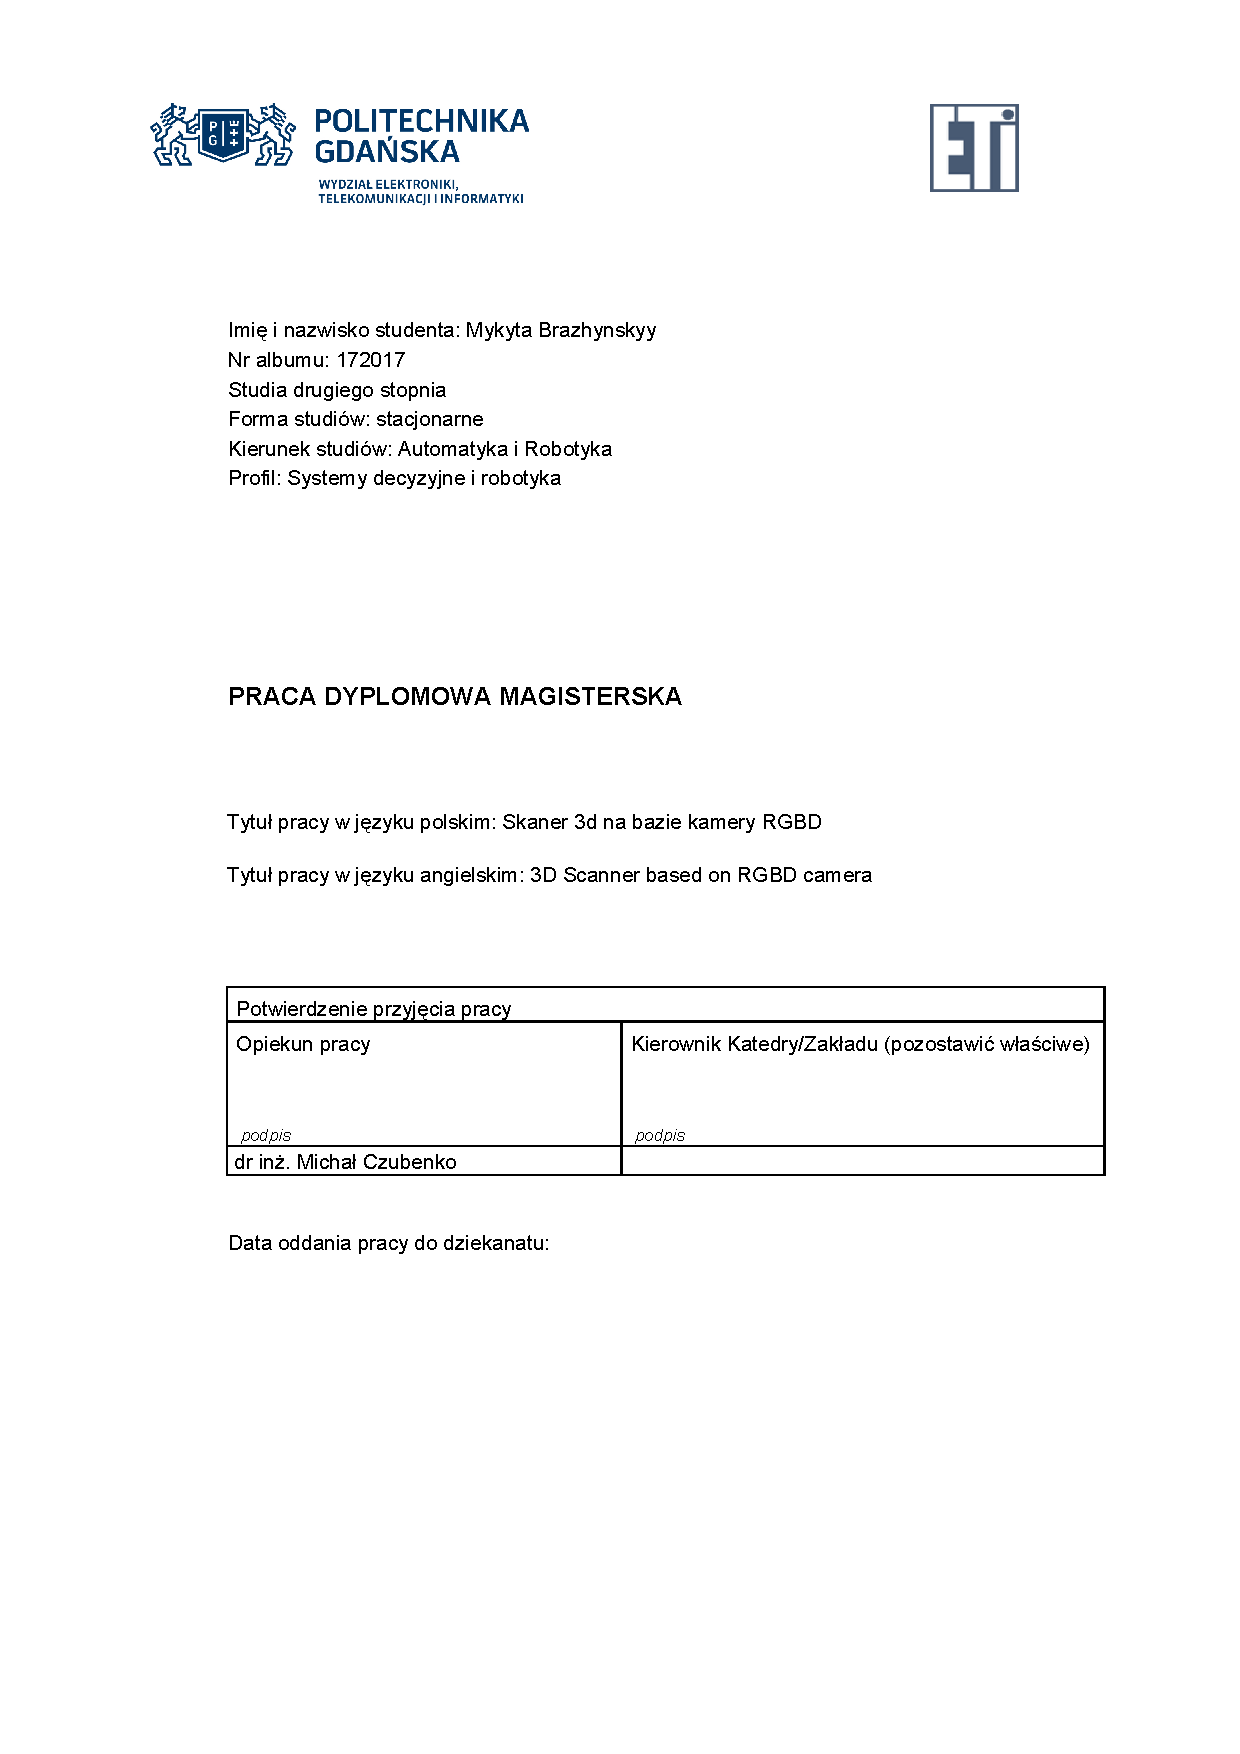
\includepdf[pages=-]{tytolowanowa.pdf}
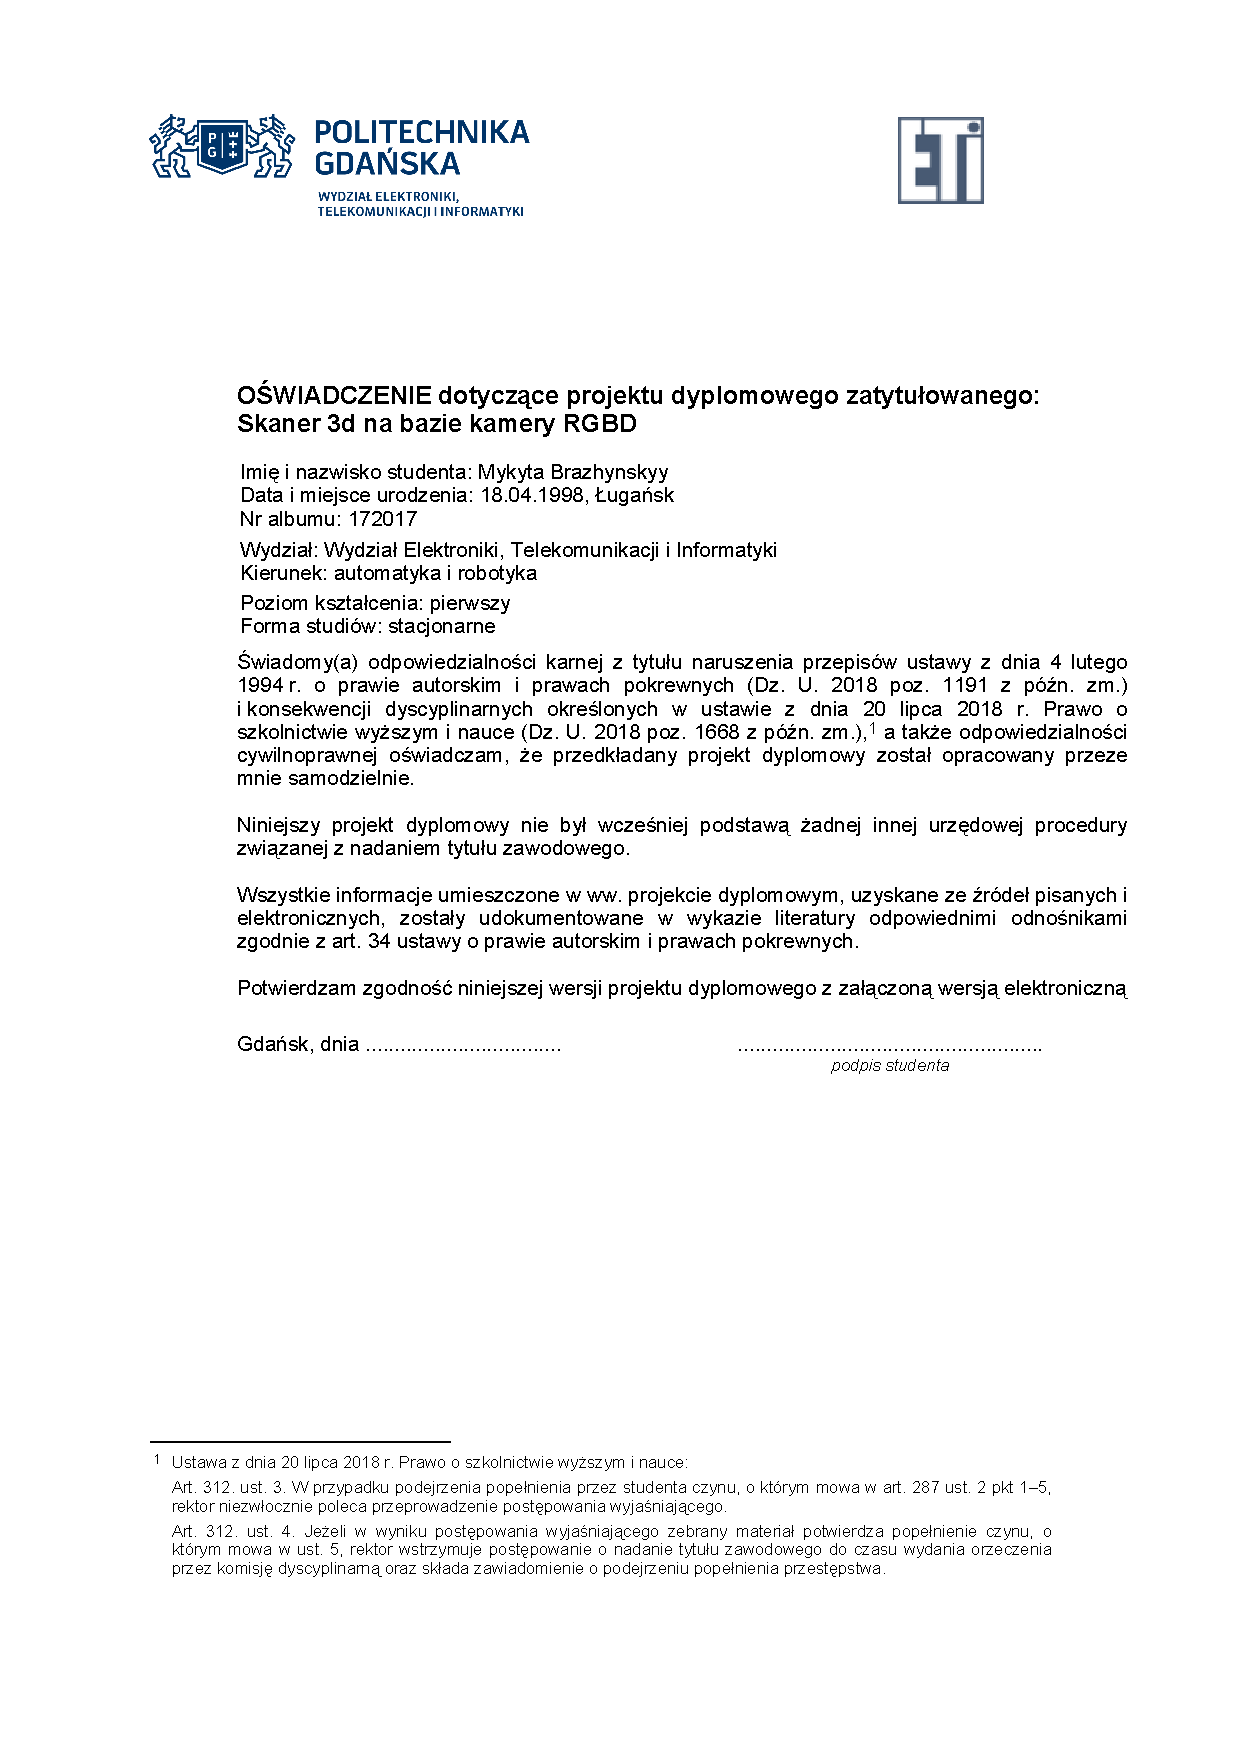
\includepdf[pages=-]{oswiadczenie.pdf}


\setcounter{page}{3}

 
\section*{STRESZCZENIE}
Celem niniejszej pracy dyplomowej było stworzenie skanera 3D oraz systemu wizualizacji utworzonych modeli rzeczywistych obiektów. Do budowy urządzenia wykorzystano kamerę głębi firmy Intel o nazwie RealSense D435i. W pracy został przedstawiony sposób budowy skanera 3D, jego kalibracji oraz algorytmy służące do przetwarzania otrzymanych danych pomiarowych w celu uzyskania wirtualnych modeli. W celu łatwiejszej obsługi programu został utworzony interfejs graficzny zawierający najważniejsze parametry wizualizacji i obróbki danych. Na koniec dane są eksportowane do modeli w formacie obsługiwanym przez program Blender.

\keywordspl{Skaner 3D ,Intel RealSense, Python, Kamera RGBD}

\dnauki{Nauki inżynieryjne i techniczne, Systemy automatyzacji i kontroli }

\section*{ABSTRACT}
The aim of this thesis was to create a 3D scanner and a system for visualization of created models based on real objects. In the work is presented how to build a 3D scanner, its calibration and algorithms used to process the obtained measurement data to obtain virtual models. In order to make the program easier to use, a graphic interface was created containing the most important parameters of visualization and data processing. Finally, the data are exported to the models in a format supported by the Blender program.

\keywordseng{3D Scanner, Intel RealSense, Python, RGBD Camera}
\newpage
\tableofcontents


\newpage

\chapter*{WYKAZ WAŻNIEJSZYCH OZNACZEŃ I SKRÓTÓW}
\subsection*{RGB}
Paleta barw tworząca kolor piksela. Oznaczenie pochodzi od kolorów Red, Green, Blue czyli czerwony, zielony, niebieski.
\subsection*{Kamera RGBD}
Kamera głębi, oprócz wykonywania zdjęć RGB potrafi ona również dokonać pomiaru odległości od obiektów i nanieść te informację na powierzchnię poszczególnych pikseli obrazu.
\subsection*{LIDAR}
Ang.(Light Detection And Ranging) urządzenie służące do dokładnego pomiaru odległości. Działaniem przypomina funkcjonowanie radaru, lecz korzysta z odliczania czasu przelotu światła lasera, a nie mikrofal.
\subsection*{Blender}
Oprogramowanie służące do modelowania trójwymiarowego.Posiada szereg funkcji do animacji obiektów, generacji tekstur oraz importowania i eksportowania gotowych modeli.
\subsection*{Maya}
Program komputerowy, umożliwiający generację zaawansowanych modeli 3D przeznaczony do zastosowań przemysłowych. W tym programie zostały stworzone filmy takie jak Spiderman, Avatar oraz Up.
\subsection*{LIDAR}
Skaner impulsowy LIDAR jest urządzeniem mierzącym odległość za pomocą wiązki światła. Jego zasada działania jest zbliżona do funkcjonowania radaru.
\chapter{WSTĘP I CEL PRACY}
\section{Wprowadzenie}
W bieżącym rozdziale przedstawione zostaną wyniki implementacji dwóch metod rekonstrukcji powierzchni z chmury punktów. Omówione zostaną charakterystyki poszczególnych algorytmów oraz rezultaty dzięki nim uzyskane. Ukazana zostanie implementacja wybranego z nich.
W celu uzyskania trójwymiarowych modeli na podstawie skanów rzeczywistych obiektów, przetestowano dwie metody generacji meshu. Pierwszą z nich jest ball pivoting algorithm. Kolejnym algorytmem będzie trójwymiarowa triangulacja Delaunay'a.


\section{Cele i założenia}
Celem niniejszej pracy jest zaprojektowanie skanera 3D korzystającego z metody triangulacji laserowej  oraz wyeksportowanie modeli do programu Blender przy zastosowaniu kamery RGBD. Projekt składa się z dwóch części, budowy skanera trójwymiarowego oraz stworzenie programu do obróbki otrzymanych danych. Odległość z jakiej będzie wykonywany skan wynosi do 1 m. Powyżej tej wartości gęstość punktów będzie zbyt niska do wiernego odtworzenia modelu. Czas trwania obliczeń w programie wynosi poniżej 15 minut. Utworzony model powinien jak najwierniej oddawać wygląd rzeczywistego obiektu, luki w teksturze powinny nieznacznie wpływać na ostateczny wygląd.

\section{Zawartość pracy}
Pierwszy rozdział opisuje cele oraz założenia pracy.Dokonano gruntownej analizy problemu, który zostanie rozwiązany w dalszym ciągu pracy.

W drugim rozdziale wykonano przegląd istniejących metod mających na celu generację trójwymiarowych obiektów na podstawie danych z kamery głębi. Dokonano porównania pomiędzy dostępnymi na rynku skanerami 3D bazującymi na różnych technologiach pomiarowych. Wymieniono ich parametry techniczne. Zobrazowano w jakich warunkach dana metoda pomiarowa powinna zostać wykorzystana. Ukazane zostały również technologie jakimi posługiwano się w przeszłości do generacji trójwymiarowych modeli. Na koniec przedstawione zostały zastosowania współczesnych skanerów 3D.

W kolejnym rozdziale przedstawiony jest model oraz konstrukcja skanera 3D. Wyjaśniono metody służące do przetworzenia danych uzyskanych z kamery głębi w chmurę punktów. Przedstawiono koncepcje istniejących rozwiązań służących do rekonstrukcji powierzchni oraz kształtu obiektów z chmury punktów.

Czwarty rozdział przedstawia podsumowanie zarówno wykonanej pracy, jak i otrzymanych efektów. Ukazane zostaną również metody analizy oraz obróbki danych, które mają posłużyć do cyfrowej implementacji rzeczywistych obiektów zarejestrowanych przez kamerę RGBD. Przedstawiono opisy zastosowanych algorytmów oraz kolejność ich wykonywania na podstawie autorskiego programu w języku Python. Poddano analizie pod względem dokładności rezultaty pomiarów w porównaniu do rzeczywistych wartości mierzonych.

Ostatni rozdział porusza kwestię potencjalnych możliwości udoskonalenia urządzenia.

\section{Wprowadzenie}
W bieżącym rozdziale przedstawione zostaną wyniki implementacji dwóch metod rekonstrukcji powierzchni z chmury punktów. Omówione zostaną charakterystyki poszczególnych algorytmów oraz rezultaty dzięki nim uzyskane. Ukazana zostanie implementacja wybranego z nich.
W celu uzyskania trójwymiarowych modeli na podstawie skanów rzeczywistych obiektów, przetestowano dwie metody generacji meshu. Pierwszą z nich jest ball pivoting algorithm. Kolejnym algorytmem będzie trójwymiarowa triangulacja Delaunay'a.


\begingroup
\newpage

\let\clearpage\relax
\chapter{Model skanera oraz koncepcja działania}
\section{Wprowadzenie}
W bieżącym rozdziale przedstawione zostaną wyniki implementacji dwóch metod rekonstrukcji powierzchni z chmury punktów. Omówione zostaną charakterystyki poszczególnych algorytmów oraz rezultaty dzięki nim uzyskane. Ukazana zostanie implementacja wybranego z nich.
W celu uzyskania trójwymiarowych modeli na podstawie skanów rzeczywistych obiektów, przetestowano dwie metody generacji meshu. Pierwszą z nich jest ball pivoting algorithm. Kolejnym algorytmem będzie trójwymiarowa triangulacja Delaunay'a.


\section{Model i konstrukcja skanera 3D}
W celu wykonania dokładnych modeli trójwymiarowych został utworzony skaner 3D na podstawie autorskiego projektu. W skład zestawu wchodzi kamera Intel RealSense D435i oraz platforma ruchoma. Wybór sensora od firmy Intel nie był przypadkowy. Posiada on szereg wbudowanych funkcji, takich jak łatwa możliwość kalibracji oraz nastaw odpowiednich parametrów wykrywania głębi. Podczas budowy skanera dokonano porównania możliwości dwóch kamer trójwymiarowych: Intel RealSense D435i oraz Orbbec Astra Mini MX6000. Porównanie charakterystyk tych produktów znajduje się w tabeli ~\ref{tab:intelvsorbbec}.

\begin{table}[H]
\begin{center}

\caption{\label{tab:intelvsorbbec}Porównanie charakterystyk kamer Intel RealSense D435i oraz Orbbec Astra Mini MX6000 \cite{OrbbecAstraMiniSheet} \cite{IntelRealSenseSheet}.}
\centerline{
\begin{tabular}{ |c| c|c| }
 \hline
 {\small Kamera} & {\small Astra Mini} & {\small RealSense D435i}\\ 
 \hline
 {\small Dokładność} & {\small $\pm$ 1-3mm na 1 m} & {\small < \text{2\%}  na 2 m}\\ 
  \hline
   {\small FOV} & {\small 60 \degree H x 49.5 \degree V} & {\small 87 \degree H x 58 \degree V}\\ 
  \hline
 {\small Rozdzielczość RGB } & {\small 640 px x 480 px } & {\small 1920 px x 1080 px}   \\  
  \hline
   {\small Rozdzielczość głębi } & {\small 640 px x 480 px } & {\small 1280 px x 720 px }   \\  
  \hline
     {\small FPS } & {\small 30} & {\small 90}   \\  
  \hline
   {\small  Długość fali lasera } & {\small 830 nm} & {\small 850 nm}  \\  
  \hline


\end{tabular}
}

\end{center}
\end{table}
Z powyższych charakterystyk wynika, że kamera firmy Intel jest dokładniejsza oraz lepiej spełni zadanie wiernego odwzorowania modelu 3D. Ponadto oprogramowanie dostarczane przez firmę Intel o nazwie RealSense Viewer pozwala na łatwą obsługę tego urządzenia. Jest tam możliwość podglądu obrazu z kamery zarówno w 2D jak i w 3D. Można ustawić poszególne parametry niezbedne do poprawnej rejestracji obrazu takie jak moc lasera, wartość graniczną wykrywanej głębi oraz ekspozycję. Wszystkie te aspekty znacząco usprawniają proces kalibracji,produktywność oraz wpływają na poprawę dokładności generowanych obrazów.
Konstrukcja zbudowanego skanera została zaprezentowana na rysunku ~\ref{fig:konstrukcjaModelu}. 
\begin{figure}[H]
  \centering
    \includesvg[scale=0.75]{modelSkanera.svg}

  \caption{Schemat budowy autorskiego skanera 3D.}   
  \label{fig:konstrukcjaModelu}
\end{figure}
Na powyższym rysunku dostrzec można dostrzec dwa kluczowe elementy wchodzące w skład skanera. Platforma ruchoma napędzana silnikiem elektrycznym zapewnia stałą prędkość kątową obrotu tacki. Dzięki temu wyznaczanie położenia obiektu w przestrzeni jest dokładne. Wykonane zostały testy platformy napędzanej silnikiem elektrycznym oraz tej poruszanej ręcznie. Z wytworzonych w ten sposób modeli wynika jasno, iż stała prędkość kątowa obiektu jest kluczowa do poprawnego przekształcenia modelu. Kolejnym elementem wykorzystanym przy budowie skanera jest kamera RGBD. Wykonuje ona zdjęcia RGB oraz głębi z określoną częstotliwością oraz zapisuje je do pliku, w celu późniejszej ich obróbki. Dokonane zostało porównanie wpływu FPS na wygląd ostatecznego modelu. Bezpośrednio wpływa to na rozdzielczość kątową wykonanych zdjęć, a co za tym idzie, zmniejszenie gęstości chmury punktów.\\
Skaner funkcjonuje w następujący sposób:
\begin{enumerate}
    \item Mierzona jest dokładna odległość obiektywu kamery od środka tacki.
    \item Obiekt umieszczany jest na obrotowej tacce.
    \item Dokonuje się kalibracji tak ustawionego elementu, tak by stopień wypełnienia punktów był jak najdokładniejszy.
    \item Tacka zostaje uruchomiona z prędkością 0.1 $\frac{rad}{s}$.
    \item Uruchomiony zostaje zapis obrazu głębi oraz RGB z kamery.
    \item Gdy tacka wykona pełen obrót, nagrywanie oraz tacka zostają zatrzymane.
\end{enumerate}

Wysokość obiektu jest mierzona na podstawie danych z kamery RGBD. Znając odległość kamery od obiektu, można wyznaczyć jego wysokość korzystając ze wzoru.

\begin{equation}
    \begin{aligned}
        H=\frac{163.6}{3.7 \cdot D} -10.6
    \end{aligned}
\end{equation}

Powyższy wzór został wyznaczony metodą empiryczną. W tym celu zmierzono wysokość obiektu na obrazie kamery oraz odległość od tego obiektu od obiektywu. Badanie powtórzono dwanaście razy w celu uzyskania dokładnej liniowej aproksymacji. Następnie wyznaczona została linia najlepszego dopasowania, wykorzystując również informację o tym, że powinna to być zależność odwrotnie proporcjonalna. Wykres przedstawiający zmierzone punkty oraz linię będącą wynikiem metody najmniejszych kwadratów ukazany na rysunku ~\ref{fig:wysokoscOdleglosc}.
\begin{figure}[H]
  \centering
    \includesvg[scale=0.75]{wysokosc_odleglosc}

  \caption{Zależność wysokości w pikselach od odległości kamery od obiektu.}   
  \label{fig:wysokoscOdleglosc}
\end{figure}

\section{Przejście do chmury punktów}
Przypomnieć zasade działania skanera i jak to wykorzystujemy. Tutaj pokazujemy na jakiej zasadzie następuje przejście z płaszczyzny 2D do 3D.Dać obrazek zastosowanej metody oraz równania.

Metoda przejścia w chmurę punktów na podstawie danych z kamery RGBD składa się z kilku kroków. Poniżej zostały opisane procedury, które należy wykonać w celu otrzymania wyżej wymienionego rezultatu.
\subsection{Wstępna obróbka danych.}
Pierwszym krokiem użytej metody jest wstępna obróbka danych. Odczytywane są dane zapisane w pliku .bag z kamery RGBD. Następnie, wybierana jest kolumna obrazu która posłuży do ekstrakcji danych z kamery głębi. Filtracja w ten sposób danych ma na celu zwiększenie wydajności kodu. Dzieje się tak, ponieważ do późniejszych algorytmów będzie wykorzystywana tylko jedna kolumna z klatki obrazu,a nie cały obraz.

\subsection{Przekształcenie danych z kamery RGBD do współrzędnych 3D.}
Następnym etapem schematu jest przejście z dwuwymiarowego układu współrzędnych kamery do trójwymiarowego układu obiektu. W tym celu zostanie użyte poniższe przekształcenie, wynikiem którego będzie macierz czterowymiarowych punktów. W skład punktu wchodzą trzy współrzędne odpowiadające pozycji w przestrzeni oraz wartość RGB danego punktu symbolizująca jego kolor.

\begin{equation}
    \begin{aligned}
            & D_{\beta}=\begin{bmatrix}d_{0} & \dots & d_{max} \end{bmatrix}  \\
            & RGB_{\beta}=\begin{bmatrix}rgb_{0} & \dots & rgb_{max} \end{bmatrix}  \\
            & X_{\beta}=cos(\beta)(R-D_{\beta})  \\
            & Y_{\beta}=sin(\beta)(R-D_{\beta})  \\
          & Z=\begin{bmatrix} 0 & \dots & H_{max} \end{bmatrix}  \\
          & w_{\beta}^n=\begin{bmatrix} X_{\beta}[n] & Y_{\beta}[n] & Z[n] & RGB_{\beta}[n]\end{bmatrix}  \\
    \end{aligned}
    \label{equ:chmuraPunktow}
\end{equation}

$\beta$ jest kątem obrotu tacki. R jest odległością obiektywu kamery od środka osi obrotu tacki. $D_{\beta}$ to macierz zmierzonych odległości punktów na płaszczyźnie obiektu od kamery dla danego kąta obrotu $\beta$. $X_{\beta}$,$Y_{\beta}$ są macierzami współrzędnych punktów na osi X,Y dla nago kąta $\beta$. $H_{max}$ to wysokość obiektu. Z to macierz współrzędnych punktów na osi Z. Wypełniona jest ona punktami z zakresu od 0 do $H_{max}$. $w_{\beta}^n$ to współrzędne n-tego punktu w płaszczyźnie XYZ dla danego kąta obrotu $\beta$.

\subsection{Normalizacja otrzymanych punktów.}
Kamera RGBD jest zaawansowanym technicznie urządzeniem. Pomimo kalibracji kamery, w przechwyconych obrazach mogą występować niedoskonałości. Przejawiają się one w złych pozycjach punktów względem pozostałych wartości. Jest to spowodowane błędnymi odczytami głębi poprzez sensor kamery i jest nieuniknione. Można jedynie sprawić, by ten błąd był jak najmniejszy. Normalizacja takich punktów sprowadza się do zbadania, czy owy punkt leży w odległości od środka podobnej do jego sąsiadów. W tym celu została wyznaczona średnia odległość punktów od osi przechodzącej przez środek obrotu tacki, która ma współrzędne (0,0,H). Warto zauważyć, że wartość współrzędnej Z nie pływa na wyznaczanie odległości, ponieważ utworzona ona została na podstawie równomiernego rozkładu wartości wysokości danego obiektu. Następnie, znając wartość średniej odległości punktów od środka układu współrzędnych, można empirycznie dobrać wartość graniczną odległości powyżej której punkty będą poddane interpolacji.

\subsection{Interpolacja punktów}
Interpolacja jest procesem aproksymacji współrzędnych punktów w miejscach, w których wystąpiły przekłamania. Jest wiele różnych metod interpolacji, które mają za zadanie jak najwierniej oddać wartość punktu w nieznanym miejscu. Głównymi metodami są metoda najbliższych sąsiadów oraz interpolacja wielomianowa.

\paragraph{Metoda najbliższych sąsiadów.\newline}\\
Interpolacja korzystająca z metody najbliższych sąsiadów jest często stosowanym algorytmem do rekonstrukcji danych w nieznanym miejscu. Wykorzystywana jest na przykład przy powiększaniu zdjęć do uzyskania lepszej rozdzielczości \cite{han2013comparison}. Zasada działania tej metody została przedstawiona poniżej.
\begin{enumerate}
    \item Wybierany jest punkt P, którego wartość ma zostać uzyskana.
    \item Mierzona jest odległość tego punktu od 4 punktów z nim sąsiadujących. Jeśli współrzędne punktu są dwuwymiarowe to odległość od sąsiada $D_{n}$ może zostać wyliczona za pomocą wzoru 
    \begin{equation}
             D_{n}=\sqrt{(x_{p}-x_{n})^2+(y_{p}-y_{n})^2}    \\
\end{equation}
$x_{p},y_{p}$ są współrzędnymi punktu, a $x_{n},y_{n}$ są współrzędnymi n-tego sąsiada.
    \item Punktowi przypisywana jest wartość sąsiada, którego odległość od niego jest najmniejsza.
\end{enumerate}
\paragraph{Interpolacja wielomianowa.\newline}\\
Interpolacja wielomianowa jest szeroko stosowanym zagadnieniem w matematyce oraz fizyce. Jej szczególnymi odmianami są interpolacja liniowa oraz kwadratowa. Polega ona na dopasowaniu funkcji na przykład liniowej,kwadratowej lub dowolnego innego wielomianu do zbioru punktów. Znając funkcję przechodzącą przez wszystkie punkty ze zbioru, można określić jaka będzie jej wartość w punkcie którego wartość była dotychczas nieznana. Równania przedstawiające tę metodę zostały przedstawione poniżej.
\begin{equation}
    \begin{aligned}
            &X=\begin{bmatrix}
                    x_{0}^0 &\dots & x_{0}^n\\
                     \vdots  & \ddots & \vdots \\
                    x_{n}^0 &\dots & x_{n}^n
                \end{bmatrix}\\
            &A=\begin{bmatrix}
                    a_{0}\\
                      \vdots \\
                    a_{n}
                \end{bmatrix}\\
            &Y=\begin{bmatrix}
                y_{0}\\
                  \vdots \\
                y_{n}
            \end{bmatrix}\\
            &Y=X \cdot A\\
            &A=X^{-1} \cdot Y\\
            & W(x)=a_{0}+a_{1}\cdot x +a_{2}\cdot x^2+\ldots +a_{n}\cdot x^n
    \end{aligned}
    \label{equ:wielomianowaEqu}
\end{equation}

X jest macierzą współrzędnych x ze zbioru dostępnych punktów. A jest macierzą współczynników wielomianu W(x). Y jest macierzą współrzędnych y ze zbioru dostępnych punktów. W(x) jest wielomianem przechodzącym przez wszystkie punkty ze zbioru.

Znając wielomian interpolacyjny można określić współrzędne poszukiwanego punktu, który znajdował się poza zbiorem dostępnych punktów, jego współrzędne to P($x_{p}$,$W(x_{p})$)

\section{Rekonstrukcja powierzchni}
Wszystkie powyższe metody pozwalały na określenie chmury punktów danego obiektu. W celu wyeksportowania gotowego modelu, potrzebna jest również znajomość całej powierzchni danego przedmiotu. W tym pomocne okazują się różne metody rekonstrukcji powierzchni. Jest to kluczowy element działania algorytmu wirtualizacji rzeczywistych obiektów do postaci modeli 3D. Powstało wiele prac naukowych na temat różnych metod rekonstrukcji powierzchni, poniżej zostały omówione najważniejsze z nich.
\subsection{Trójwymiarowa triangulacja Delaunaya}
Triangulacja powierzchni metodą Delaunaya jest jedną z popularniejszych metod nakładania siatki na nieregularnie rozprowadzone punkty. Polega ona na połączeniu punktów w nieprzecinające się trójkąty, dzięki czemu możliwe jest nałożenie na nie koloru oraz utworzenie meshu na danym obiekcie. Triangulację Delaunaya można wykonać dla dowolnej N-wymiarowej płaszczyzny, w danym przykładzie zostanie opisana metoda dla trójwymiarowej chmury punktów \cite{cignoni1998dewall}. Schemat działania tej metody został opisany poniżej. 
\begin{enumerate}
    \item Tworzony jest czworościan zawierający wszystkie punkty ze zbioru.
    \item Tworzona jest lista czworościanów do usunięcia oraz czworościanów do pozostawienia.
    \item Dla każdego punktu sprawdzane jest czy leży on wewnątrz sfery opisanej na czworościanie do pozostawienia. Jeśli leży,to tworzone są 4 czworościany z wierzchołków starego oraz z nowego punktu.
    \Item Na końcu początkowy czworościan wewnątrz którego znajdowały się wszystkie punkty zostaje usunięty. Skasowane zostają również wszystkie czworościany mające z nim wspólny wierzchołek.
\end{enumerate}
Zaletą tej metody jest to, że jest ona inkrementacyjna. Punkty do triangulacji są dodawane po kolei,a co za tym idzie, nie ma potrzeby tworzenia nowej siatki po dodaniu pojedynczego punktu. Wystarczy jedynie wykonać jedną fazę algorytmu i dopisać utworzone wierzchołki czworościanów do listy.
Modyfikacją tej metody jest triangulacja DeWall zaproponowana przez włoskich naukowców w 1997 roku \cite{cignoni1998dewall}. Jej nazwa pochodzi od Delaunay i ściana (ang. \textit{Wall}). Pojęcie ściany oznacza w tym wypadku rekurencyjne dzielenie zbioru punktów na dwa podobne do siebie obszary, następnie równoległe utworzenie dwóch niezależnych od siebie triangulacji Delaunaya. Dzięki podzieleniu zbioru punktów na niezależne od siebie obszary, możliwe staje się wykorzystanie wielowątkowości procesora do obliczeń równoległych. To znacząco przyspiesza pracę algorytmu.
\subsection{Algorytm maszerujących sześcianów}
Algorytm maszerujących sześcianów jest metodą typu dziel i podbijaj zaproponowaną w 1987 roku przez amerykańskich naukowców w Nowym Yorku \cite{lorensen1987marching}. W przeciwieństwie do triangulacji Delaunaya, punkty na które ma zostać nałożona siatka meshu muszą być w regularnych odstępach od siebie. W związku z tym, chcąc wykorzystać tę metodę trzeba dokonać interpolacji punktów, w celu przejścia z nieregularnych przestrzeni pomiędzy elementami do równomiernie leżących punktów. Ze względu na schemat działania algorytmu, jest on niezwykle szybki, ponieważ pozwala on na uniknięcie części obliczeń. Algorytm dzieli przestrzeń na regularne sześciany, a następnie sprawdza przecięcia punktów ze ścianami sześcianu. Przy regularnej siatce punktów istnieje $2^8$ takich przecięć, ponieważ sześcian ma 8 krawędzi, na każdej z nich może leżeć punkt lub nie. Po uwzględnieniu symetrii obrotowej sześcianu liczbę kombinacji można zredukować do zaledwie 15. Zostały one przedstawione na rysunku ~\ref{fig:marchingCubesCut}.
\begin{figure}[H]
  \centering
  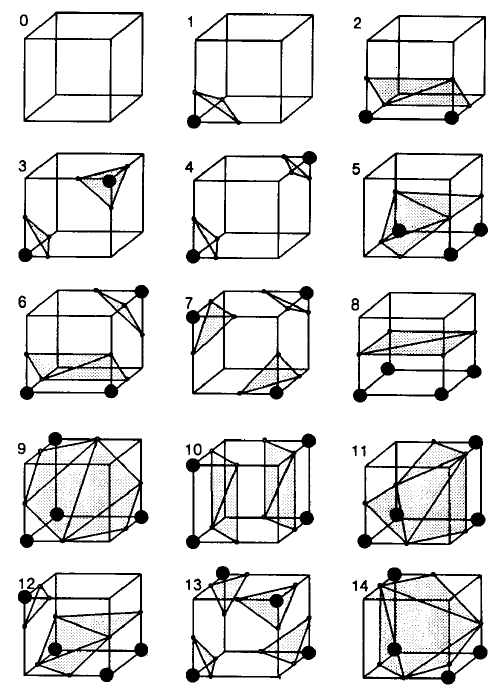
\includegraphics[scale=0.5]{przeciecia.PNG}
  \caption{Możliwe przecięcia sześcianu przez punkty \cite{lorensen1987marching}}   
  \label{fig:marchingCubesCut}
\end{figure}
Przecięcia punktów z sześcianami tworzą trójkąty, które później zostaną dodane do triangulacji. Należy zwrócić uwagę na to, że gęstość meshu na obiekcie poddanym triangulacji bezpośrednio zależy od długości boku sześcianu. Im jest on mniejszy, tym więcej będzie przecięć punktów z krawędziami, a co za tym idzie, więcej utworzonych trójkątów triangulacyjnych. Występują odmiany tej metody wprowadzające zmienną długość boku danego sześcianu \cite{shu1995adaptive}. Adaptacyjna metoda maszerujących sześcianów bada krzywiznę powierzchni wewnątrz sześcianów za pomocą wyznaczania wektorów normalnych utworzonych dla danych trójkątów. Jeśli wektory odchylone są w podobną stronę, oznacza to, że powierzchnia jest dostatecznie gładka. W przeciwnym wypadku sześcian dzielony jest na kolejne 8 sześcianów i algorytm jest powtarzany do momentu uzyskania odpowiedniej krzywizny powierzchni. Dzięki wykorzystaniu tej metody tworzona jest dokładniejsza triangulacja powierzchni względem początkowego algorytmu. Ponadto dzięki wykorzystaniu adaptacyjnej metody algorytm jest szybszy niż ten który by miał ustalona długość boku. Porównanie algorytmu maszerujących sześcianów oraz jej adaptacyjnej odmiany dla różnych ilości punktów znajduje się w tabeli ~\ref{tab:amcvsmc}.

\begin{table}[H]
\begin{center}
\caption{\label{tab:amcvsmc}Porównanie algorytmu MS oraz adaptacyjnych MS dla 7.4\cdot $10^6$ oraz 2.8\cdot $10^6$ punktów \cite{shu1995adaptive}.}
\begin{tabular}{ |c| c|c|c|c| }
 \hline
 {\small Metoda} & {\small MS}&{ \small AMS} & {\small MS}&{ \small AMS}\\ 
  \hline
     {\small Liczba punktów } & {\small  7.4\cdot $10^6$ } & {\small  7.4\cdot $10^6$ } & {\small  2.8\cdot $10^6$ } & {\small  2.8\cdot $10^6$ }   \\  
  \hline
     {\small Czas trwania } & {\small 331 s} & {\small 230 s}& {\small 164 s} & {\small 81 s}    \\  
  \hline
   {\small  Ilość trójkątów } & {\small 718964 } & {\small 299292 }& {\small 393606 } & {\small 102868 }  \\  
  \hline
\end{tabular}
\end{center}
\end{table}



\subsection{Ball pivoting algorithm}

Algorytm toczącej się kuli jest metodą służącą do rekonstrukcji powierzchni na podstawie chmury punktów. Został on zaproponowany przez Fausto Bernardini i pozostałych w 1999 roku \cite{bernardini1999ball}. BPA został stworzony by szybko i dokładnie odwzorowywać kształt powierzchni. Schemat postępowania programu, opiera się o kulę, która toczy się po powierzchni punktów. Z początku, wybierany jest pierwszy trójkąt triangulacyjny. Trzy punkty utworzą pierwszy trójkąt triangulacyjny, jeśli kula styka się tylko i wyłącznie z nimi. Gdy tocząc się ,kula natrafi na dodatkowy punkt, to zostaje on połączony z bokiem wcześniejszego trójkąta. Cały proces powtarza się do momentu, gdy kula pokona całą powierzchnię. Pomimo przejścia kuli przez całą powierzchnię, nie oznacza to, że ze wszystkich punktów zostanie utworzony mesh. Warto nadmienić, że głównym parametrem wpływającym na czas trwania algorytmu jest promień kuli. W większości przypadków, ustala się go na podstawie średniej odległości punktów od siebie. Jeśli promień będzie niedostatecznie duży, to kula może "wypaść" przez punkty, więc nie zostaną one połączone. Powstają wtedy dziury, które negatywnie wpływają na ostateczny wygląd meshu. Można je później załatać wykorzystując algorytmy interpolacji liniowej lub ponownie uruchomić algorytm BPA, tym razem z większym promienień i powtórzyć cały proces jeszcze raz. W efekcie czego większość dziur zostanie załatana. Wpłynie to jednak negatywnie na czas trwania algorytmu. Wizualizacja zasady działania algorytmu została przedstawiona na rysunku ~\ref{fig:bpaZasada}

\begin{figure}[H]
  \centering
  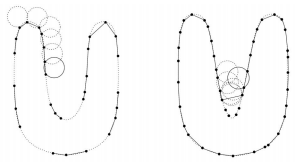
\includegraphics[scale=0.8]{bpa_zasada.PNG}
  \caption{Zasada działania algorytmu BPA \cite{bernardini1999ball}}   
  \label{fig:bpaZasada}
\end{figure}
Główną zaletą przy wykorzystaniu tego algorytmu jest fakt, że jego złożoność obliczeniowa zależy liniowo od ilości punktów w zbiorze. Jeśli dodamy dodatkowy punkt, to kula musi się przez niego przetoczyć kilka razy. Jednak cała struktura pozostałych punktów pozostaje niezmienna. Ten aspekt algorytmu stanowi największą odmianę względem triangulacją Delaunay'a. W triangulacji Delaunay'a, po dodaniu dodatkowego punktu cała struktura triangulacji może się zmienić. Ważną zaletą algorytmu jest możliwość regulacji promienia kuli R, im promień jest mniejszy, tym algorytm zajmie więcej czasu, ponieważ zetknie się z większą ilością punktów podczas toczenia. Zatem eksperymentując z długością promienia, można otrzymać zadowalająco dobre rezultaty w krótszym czasie. 



\endgroup
\chapter{Implementacja oraz porównanie metod}

\section{Wprowadzenie}
W bieżącym rozdziale przedstawione zostaną wyniki implementacji dwóch metod rekonstrukcji powierzchni z chmury punktów. Omówione zostaną charakterystyki poszczególnych algorytmów oraz rezultaty dzięki nim uzyskane. Ukazana zostanie implementacja wybranego z nich.
W celu uzyskania trójwymiarowych modeli na podstawie skanów rzeczywistych obiektów, przetestowano dwie metody generacji meshu. Pierwszą z nich jest ball pivoting algorithm. Kolejnym algorytmem będzie trójwymiarowa triangulacja Delaunay'a.


\section{Ogólny zarys funkcjonowania programu}
Autorski program, mający na celu przetworzenie danych ze skanera 3D w celu uzyskania modeli trójwymiarowych składa się z wielu istotnych kroków. Począwszy od wczytania danych z kamery trójwymiarowej, a skończywszy na eksportowaniu modeli do programu Blender. Istnieje wiele różnych podejść do implementacji poniższych algorytmów. Poniżej zostaną omówione autorskie metody na ich implementację oraz optymalizację. W rozdziale zostaną opisane najważniejsze algorytmy oraz ich szczegółowe charakterystyki. Program zawiera graficzny interfejs, który ma umożliwić użytkownikom łatwą obróbkę danych.
\subsection{Odczytanie danych z kamery RGBD}
Pierwszym krokiem pracy programu jest odczytanie danych z kamery trójwymiarowej. Wczytane dane są poddawane różnym obróbkom w celu usunięcia przekłamań spowodowanych złymi odczytami z czujnika głębi. Głównym tego powodem jest rozpraszanie wiązki światła na obiekcie, co uniemożliwia poprawny odczyt głębi przez skaner. Przykład takiej sytuacji został przedstawiony na rysunku \ref{fig:depthErrorImage}.
\begin{figure}[H]
\centering
\subcaptionbox{Zniekształcona głębia}%
  [.4\linewidth]{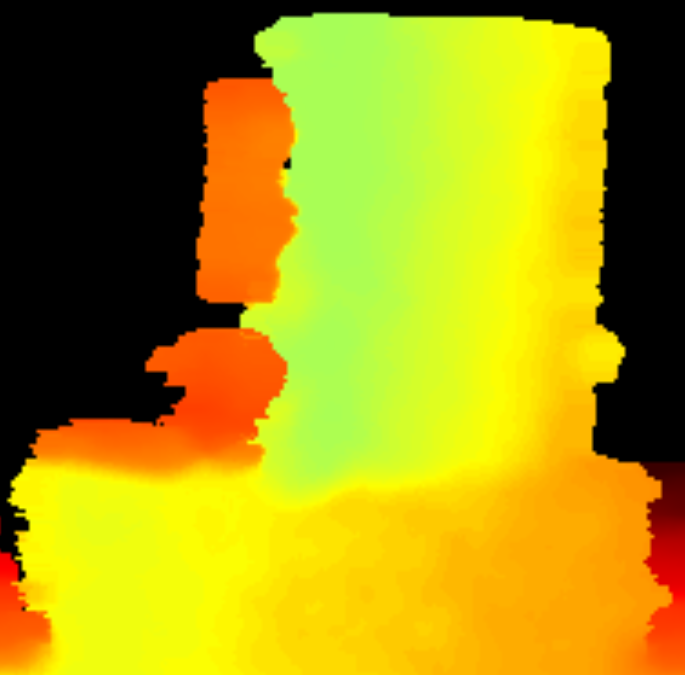
\includegraphics[height=5cm]{pudelko_glebia}}
\subcaptionbox{Głębia z nałożoną teksturą RGB}
  [.4\linewidth]{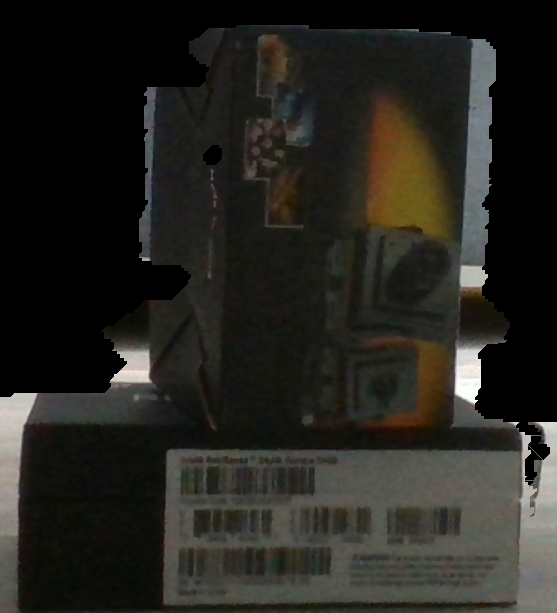
\includegraphics[height=5cm]{pudelko_kolor}}
\caption{Porównanie widoku kamery głębi oraz RGB}\label{fig:depthErrorImage}
\end{figure}
Biblioteka PyRealSense dostarczana przez firmę Intel do kamer trójwymiarowych zapewnia szereg funkcji pozwalających na oczyszczenie wynikowych danych z dziur. W pakiecie SDK zawarte są filtry chwilowe oraz przestrzenne. Filtr chwilowy umożliwia wypełnienie dziur wartościami z poprzednich klatek. Jest to funkcja, która pozwala na uzyskanie bardziej czytelnych danych. Są one również wiarygodniejsze niż użycie interpolacji do uzyskania danych. Filtr przestrzenny umożliwia wygładzenie danych zachowując jednocześnie dane brzegowe. W przypadku wcześniejszego filtru te dane są tracone w skutek mieszania danych z aktualnych oraz wcześniejszych klatek. Przydatna okazuje się również być funkcja do nakładania na siebie obrazu głębi oraz koloru. Czujnik natężenia siatki światła oraz kamera RGB znajdują się obok siebie, dlatego też piksel o współrzędnych (x,y) będzie różnił się w przypadku koloru oraz głębi \cite{IntelRealSenseSheet}. By uzyskać poprawne dane trzeba nałożyć odpowiednio klatki pochodzące z kamery RGB oraz czujnika głębi. Zostało to dokonane poprzez wykorzystanie odpowiedniej funkcji z biblioteki PyRealSense. Możliwy jest wybór względem, którego źródła mają być nakładane na siebie klatki. Na potrzeby programu klatki nakładane są na siebie względem ujęcia RGB.

Następnym krokiem jest ekstrakcja danych głębi oraz koloru ze wszystkich klatek obrazu. Porównano dwie metody akwizycji danych. W metodzie skanera liniowego brana pod uwagę jest pojedyncza kolumna z całego obrazu, zaś w metodzie światła strukturalnego przetwarzane są dane głębi pochodzące z całego obrazu. Po przeprowadzeniu należytych badań oraz analizy wyników, powstałych w skutek implementacji obu metod generacji chmur punktów, do dalszego ciągu pracy wybrano metodę skanera liniowego. Zbiór kolumn powstałych dzięki zastosowaniu tej metody posłuży w późniejszym etapie do przejścia w chmurę punktów. Wszystkie te informacje zapisywane są w pliku z rozszerzeniem npy. Ten format pliku używany jest przez bibliotekę Numpy do wykonywania szybkich zapisów binarnych danych. Dzięki temu zabiegowi, uzyskane dane z nagrania zajmują jedynie kilkanaście kB. Ten zabieg ma na celu późniejszy odczyt danych bezpośrednio z zapisanego pliku. Dzięki temu nie będzie konieczności ładowania ponownie pełnego filmu z kamery RGBD. Przekształcenie otrzymanych danych zostanie przedstawione w dalszym ciągu pracy.
\subsection{Przejście do chmury punktów}
Kolejnym istotnym krokiem algorytmu jest przejście do chmury punktów. Polega on na wyznaczeniu dla każdego dwuwymiarowego punktu, odpowiadających mu współrzędnych w przestrzeni trójwymiarowej. Przed przystąpieniem do dalszej pracy należy jednak zmierzyć odległość środka tacki, na której stał obiekt, od kamery. Jeśli ta odległość zostanie źle zmierzona, uzyskany model będzie błędny. Zostało sporządzone porównanie wpływu błędnego pomiaru na ostateczny wygląd modelu. Wszystkie modele zostały zrzutowane na płaszczyznę dwuwymiarową, ponieważ dokonywane przekształcenie nie wpływa na współrzędną Z danych punktów. Początkowa odległość kamery od środka tacki wynosiła 50 cm.

\begin{figure}[H]
\centering
\subcaptionbox{Ujemny błąd -5\%}%
  [.4\linewidth]{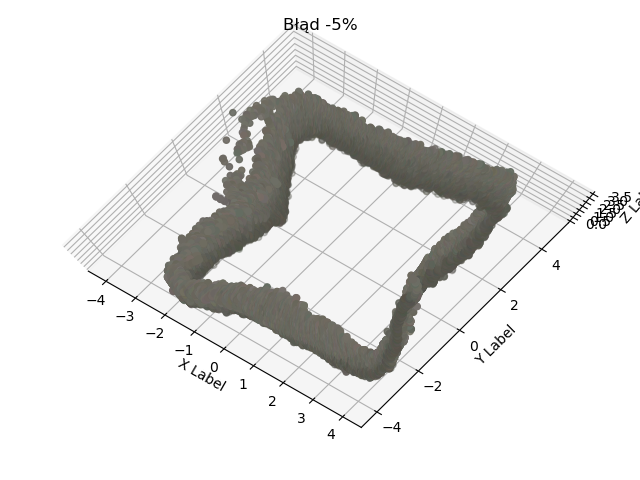
\includegraphics[height=5cm]{blad_minus5.png}}
\subcaptionbox{Ujemny błąd -10\%}
  [.4\linewidth]{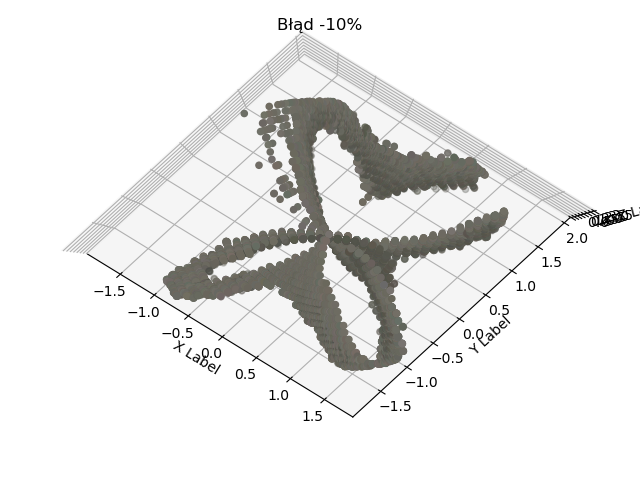
\includegraphics[height=5cm]{blad_minus10.png}}
\caption{Porównanie wpływu ujemnego błędu pomiarowego na wygląd chmury punktów dla -5\%,-10\%}\label{fig:depthErrorImageMinus}
\end{figure}

\begin{figure}[H]
\centering
\subcaptionbox{Dodatni błąd +10\%}%
  [.4\linewidth]{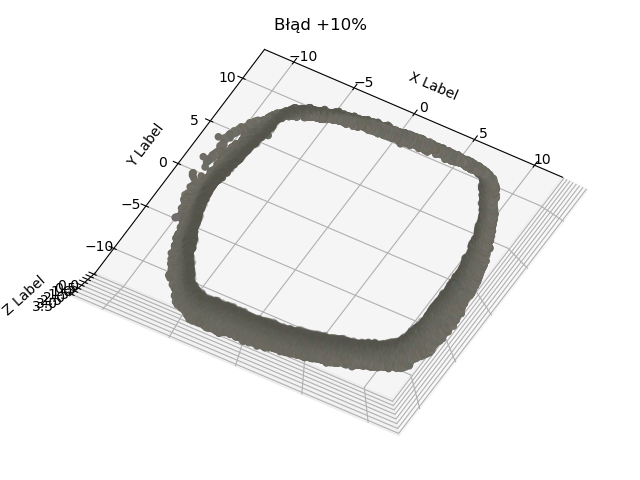
\includegraphics[height=5cm]{blad_plus10.png}}
\subcaptionbox{Dodatni błąd +20\%}
  [.4\linewidth]{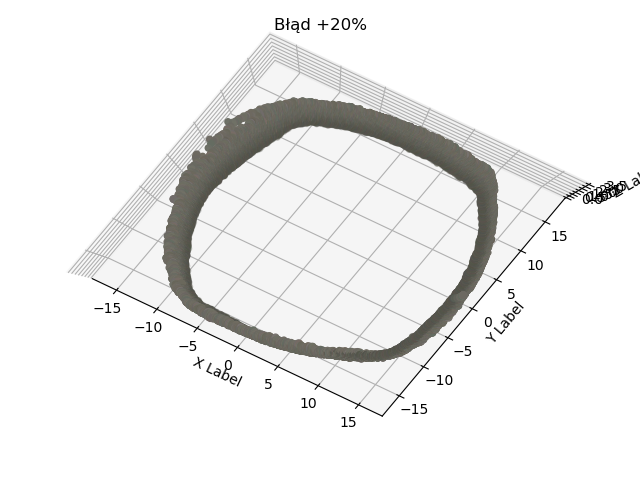
\includegraphics[height=5cm]{blad_plus20.png}}
\caption{Porównanie wpływu dodatniego błędu pomiarowego na wygląd chmury punktów dla +10\%,+20\%.}\label{fig:depthErrorImagePlus}
\end{figure}

Na rysunkach ~\ref{fig:depthErrorImageMinus} oraz ~\ref{fig:depthErrorImagePlus} można zaobserwować jak duży wpływ na ostateczny wygląd modelu ma błędne zmierzenie odległości. Jeśli stosunek błędu do rzeczywistej odległości jest większy od 1, wtedy kształt modelu przybiera formę okręgu. Jeśli zaś jest mniejszy od 1, obwód modelu zaczyna być wklęsły. Przyczyną takiego zachowania algorytmu jest wzór wykorzystywany do przejścia ze współrzędnych obiektu do współrzędnych kamery (\ref{equ:chmuraPunktow}). Ze wzoru można wywnioskować, że gdy stosunek błędnie zmierzonej odległości od środka jest o wiele większy od rzeczywistej odległości równania zaczynają opisywać współrzędne okręgu. Z kolei, przy ujemnym błędzie pomiarowym, dla $R_{b}<<R$, promień $R-D_{\beta}$ może przybierać ujemne wartości, tworząc tym samym wstęgi.
\newline \indent Kolejnym krokiem jest wyznaczenie rzeczywistej wysokości obiektu na podstawie wzoru (\ref{equ:wysokoscRealPix}). Równanie pozwala na obliczenie wysokości obiektu, znając odległość od niego oraz jego wymiary w pikselach. Znając wysokość obiektu jest możliwe ustalenie jaka powinna być gęstość punktów wzdłuż osi Z. Dzięki takiemu podejściu wymiary obiektu zostaną wiernie odwzorowane, a co za tym idzie, będzie można sprawdzić prawdziwe charakterystyki modelu. Mając informacje o rzeczywistych wymiarach, można ustalić objętość danego obiektu oraz jego powierzchnię w $m^2$.
\newline \indent Mając poprawnie wyznaczoną odległość od obiektu można przejść do wyznaczenia chmury punktów korzystając z równania ~\ref{equ:chmuraPunktow}. Do otrzymanej chmury punktów należy również dodać kolory poszczególnych pikseli uzyskane na podstawie obrazu RGB. Na potrzeby użytej metody zapisu trójwymiarowych modeli, piksele muszą zostać przeskalowane z wartości <0,255> do wartości z zakresu <0,1> dla każdego z trzech kolorów, czerwonego, zielonego oraz niebieskiego.
\subsection{Oznaczanie błędnych próbek}
Istotnym aspektem działania algorytmu jest eliminacja błędnych próbek. Jest to proces mający na celu znalezienie oraz oznaczenie przekłamanych punktów, które mogą negatywnie wpływać na ostateczny wygląd modelu. Składa się ona z kilku faz.
\newline \indent Pierwszym krokiem tej metody jest wyznaczenie średniej odległości wszystkich punktów od środka obiektu. Jest ona wyznaczana na podstawie poniższego wzoru.
\begin{equation}
    \begin{aligned}
            &D_{mean}=\frac{\sum_{n=0}^{N} \sqrt{p_{nx}^2+p_{ny}^2}}{N}  
    \end{aligned}
\end{equation}
\indent Punkt P o indeksie n posiada współrzędne $p_{nx},p_{ny}$. Zbiór na którym dokonywania jest eliminacja posiada N punktów. Średnia odległość punktu od środka układu wynosi D.
\newline \indent Warto zauważyć, że we wzorze nie występuję współrzędna Z n-tego punktu. Powodem tego jest fakt, iż punkty są równomiernie rozłożone wzdłuż osi Z. Liczenie odległości wzdłuż tej osi nie wpłynęło by na poprawienie dokładności wyznaczania odpowiednich punktów. Można więc ten etap pominąć i wykorzystać jedynie dwie pierwsze współrzędne punktu do wyznaczenia jego pozycji względem środka.
\newline \indent Dla każdego punktu ze zbioru sprawdzana jest odległość od środka. Jeśli jest ona większa, niż $p\% \cdot D_{mean}$, gdzie $p\%$ oznacza graniczny współczynnik odległości od środka, to punkt zostaje oznaczony odpowiednią flagą. Flaga umożliwia w późniejszym etapie rozpoznanie przekłamanego punktu oraz dodanie go do zbioru interpolacyjnego.
\subsection{Interpolacja punktów}
Po tym jak wszystkie przekłamane punkty zostały odpowiednio oznaczone można przejść do ich interpolacji. Wykorzystując technikę interpolacji można wyznaczyć współrzędne tych punktów, których wartości początkowo były błędne. Podczas badań otrzymanych rezultatów interpolacji, został wybrany najlepszy algorytm. Spośród interpolacji liniowej,sześciennej oraz najbliższych sąsiadów wybrana została metoda sześcienna. Daje ona najlepsze rezultaty spośród wszystkich wypróbowanych metod. Punkty zostały przekształcone za pomocą wzoru (\ref{equ:wielomianowaEqu}). Wynikiem takiej operacji jest nowa chmura punktów, która nie zawiera już przekłamanych wartości. Dzięki temu możliwe będzie dokładne utworzenie siatki triangulacyjnej na modelu. Korzystając z danej metody interpolacji uzyskane wartości mają bardziej naturalny rozkład. W przypadku jej liniowej odmiany, współrzędne punktów rosły liniowo. Sprawiało to wrażenie, że punkty na obiekcie były ułożone błędnie. Po zmianie na interpolację wielomianem trzeciego stopnia, ten problem jest niezauważalny.  
\section{Porównanie metod rekonstrukcji powierzchni}
W poniższej sekcji przedstawione zostały wyniki implementacji dwóch metod rekonstrukcji powierzchni. Dokonano porównania dokładności odwzorowania powierzchni jak również ich szczegółowości. W algorytmie BPA porównano wpływ promienia kuli na ostateczny wygląd modelu oraz czas trwania algorytmu. Dla triangulacji Delaunay'a zostanie przedstawiona szczegółowa implementacja oraz użyte metody optymalizacji. Ukazany zostanie również wpływ ilości punktów na czas trwania triangulacji.

\subsection{Algorytm BPA}
Dla porównania został zaimplementowany algorytm BPA. Jego użycie jest możliwe dzięki wykorzystaniu biblioteki Open3D. Pakiet umożliwia dokonywanie wielu operacji na chmurach punktów. Dostępne są w nim rekonstrukcje Poissona, wyznaczanie wektorów normalnych oraz dane testowe do przeprowadzania badań dokładności implementowanych algorytmów. Na potrzeby wdrożenia danej metody wykorzystana zostanie funkcja umożliwiająca stworzenie meshu przy wykorzystaniu algorytmu BPA. Implementacja algorytmu składa się z kilku kroków które zostały omówione poniżej.
\subsubsection{Estymacja normalnych}
Główną ideą algorytmu jest toczenie kuli po chmurze punktów. W przypadku kiedy gęstość 3 dotkniętych punktów jest większa od średniej gęstości to utworzony w ten sposób trójkąt będzie mniejszy. W przypadku, gdy lokalna gęstość jest jednak mniejsza niż średnia, kula może dotknąć punktu, który jest ukryty. Znajduje się on wtedy pod górną warstwą i w celu dokładnego odwzorowania powierzchni, tak utworzony trójkąt powinien zostać odrzucony \cite{mittleman1999ball}. Dana sytuacja została opisana na rysunku \ref{fig:bpaWrongTria}.
\begin{figure}[H]
  \centering
  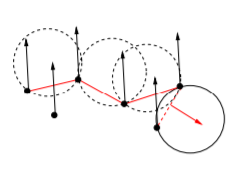
\includegraphics[scale=0.8]{bpa_wrong.PNG}
  \caption{Dotknięcie przez kule punktu pod powierzchnią \cite{mittleman1999ball}.}   
  \label{fig:bpaWrongTria}
\end{figure}

W celu wykrycia poprawnie skonstruowanego trójkąta używane są normalne. W tym celu należy obliczyć wektory normalne do powierzchni danego trójkąta oraz do średnie wektory normalne do powierzchni blisko danego trójkąta. 
\begin{equation}
    \begin{aligned} 
    \begin{cases}
            &N_{tri}=\vec{AB} \times \vec{AC}\\
            &N_{mean}=\frac{\sum_{i=1}^{K} \vec{A_{i}B_{i}} \times \vec{A_{i}C_{i}}}{K}\\
            & |N_{tri}||N_{mean}|cos(\theta)=N_{tri} \cdot N_{mean}\\
            &\theta=arccos(\frac{N_{tri} \cdot N_{mean}}{|N_{tri}||N_{mean}|})
    \end{cases}
    \end{aligned}
\end{equation}
\indent Wektorem normalnym do powierzchni trójkąta jest $N_{tri}$. Wokół trójkąta triangulacyjnego znajdują się sąsiednie trójkąty w liczbie K, tworzące uśredniony wektor normalny $N_{mean}$. Kąt pomiędzy wektorem normalnym do trójkąta, a do powierzchni wokół niego wynosi $\theta$.
\newline \indent Trójkąt interpolacyjny należy odrzucić, gdy iloczyn skalarny jego wektora normalnego oraz normalnej do powierzchni jest ujemny. Oznacza to, że kąt $\theta$ pomiędzy nimi będzie większy od $\frac{\pi}{2}$. Dla wartości powyżej 90 stopni trójkąt będzie skierowany przeciwnie do powierzchni i należy go odrzucić. Do wyznaczenia wektorów normalnych do chmury punktów użyta została funkcja dostępna w bibliotece open3D. Znajduje ona punkty w okolicy danego punktu i przecinając je prostą tworzy wektor normalny. Następnie wektory normalne do punktu są uśredniane i wyznaczane za pomocą analizy kowariancji.
\subsubsection{Wyznaczenie średniej odległości punktów}
Kolejnym krokiem potrzebnym do poprawnego funkcjonowania algorytmu BPA jest odpowiedni dobór promienia kuli R. Jest to bardzo istotny parametr algorytmu. Odpowiedni jego dobór sprawi, że wyjściowy model trójwymiarowy obiektu będzie szczegółowy i będzie zawierał mało luk. Jednakże wraz ze wzrostem długości promienia rośnie również czas obliczeniowy programu. Promień powinien być więc dobierany z uwzględnieniem obu tych aspektów. W celu jego najlepszego doboru należy wyznaczyć średnią odległość punktów od siebie. Znając tę odległość, będzie można odpowiednio dobrać długość R, by kula nie wpadała w przestrzenie pomiędzy punktami. Za obliczenie średnich odległości odpowiada funkcja z biblioteki open3D. Dla każdego punktu w chmurze wyznacza jest odległość od najbliższego sąsiada. Z tak powstałego wektora odległości można wyznaczyć średnią korzystając z biblioteki Numpy w celu optymalizacji czasu obliczeniowego. Następnie, traktując średnią odległość pomiędzy obiektami jako punkt wyjściowy, można empirycznie dobrać odpowiednią wartość promienia kuli R. W tabeli \ref{tab:bpaRInfluence} został przedstawiony wpływ wielkości promienia R na czas trwania obliczeń oraz ilość trójkątów.
\begin{table}[H] 
\begin{center}
\caption{\label{tab:bpaRInfluence}Czas trwania triangulacji metodą BPA w zależności od długości promienia R dla średniej odległości między punktami równej D_{mean}=0.047.}
\centerline{
\begin{tabular}{ |c|c|c|c| }
 \hline
 { Długość promienia} & { $\frac{R}{D_{mean}}$ }&{ Czas trwania}& { Liczba trójkątów}\\ 
  \hline
   {\small 0.047 } & {\small 1} & {\small 0.51 s}& {\small 42819}  \\  
  \hline 
     {\small 0.09 } & {\small 2} & {\small 1.44 s}& {\small 44025}  \\  
  \hline 
   {\small 0.14 } & {\small 3} & {\small 7.5 s}& {\small 32474}  \\  
  \hline 
     {\small 0.19 } & {\small 4} & {\small 29.8 s}& {\small 24936}  \\  
  \hline 
       {\small 0.23 } & {\small 5} & {\small 93 s}& {\small 21496}  \\  
  \hline 
         {\small 0.28 } & {\small 6} & {\small 215 s}& {\small 18641}  \\  
  \hline 
           {\small 0.33 } & {\small 7} & {\small 430 s}& {\small 16348}  \\  
  \hline 
             {\small 0.38 } & {\small 8} & {\small  737s}& {\small 14457}  \\  
  \hline 

\end{tabular}
}
\end{center}
\end{table}
W powyższej tabeli przedstawiony został wpływ wielkości promienia na czas obliczeń oraz liczbę trójkątów. Z danych zebranych podczas testów można wysnuć wniosek, iż wraz ze wzrostem długości promienia kuli, rośnie czas trwania algorytmu. Maleje przy tym ilość utworzonych trójkątów. Podstawą takiego zachowania jest fakt, iż przy większym promieniu kula dotyka mniejszej ilości punktów, tym samym tworząc mniej trójkątów. Jednocześnie czas trwania algorytmu rośnie, ponieważ badanie sąsiedztwa punktów zajmuje więcej czasu. Przy większym promieniu kuli, poszukiwana jest liczba sąsiadów danego punktu w większym otoczeniu. To znacząco wpływa na złożoność obliczeniową.
\newline \indent Po wyznaczeniu normalnych oraz dobraniu promienia kuli ostatnim krokiem jest utworzenie triangulacji BPA. Wykorzystując funkcję z biblioteki open3D można przeprowadzić algorytm toczącej się kuli i uzyskać ściany trójkątów triangulacyjnych. Funkcja dostępna w bibliotece jest udoskonaleniem początkowej metody zaproponowanej przez Bernardini w 1999 roku. Wprowadza ona możliwość równoległego przeprowadzania obliczeń w celu ich szybszego wykonywania \cite{digne2014analysis}. By z większą prędkością odnajdywać sąsiadujące punkty użyto również drzewa ósemkowego. Jest to struktura danych umożliwiająca podzielenie przestrzeni na mniejsze części, a następnie utworzenie drzewa sąsiedztw. Znając strukturę drzewa, można je przeszukiwać w bardzo łatwy sposób, by odnaleźć odpowiednich sąsiadów punktu. Tworzenie tej struktury ma charakter rekurencyjny. Początkowo generowany jest sześcian otaczający wszystkie punkty, następnie jest on dzielony na 4 sześciany. Każdy kolejny na kolejne 4 rekurencyjnie. Podział trwa do momentu, kiedy wewnątrz sześcianu znajduje się nie więcej niż 8 punktów. Każdy korzeń w drzewie ma 8 gałęzi. Współrzędne każdego punktu w drzewie można zapisać binarnie. Znając pozycję danego punktu w drzewie, korzystając ze wzoru oraz przesunięć binarnych można odnaleźć jego sąsiadów. Dzięki tym operacjom przeprowadzony zostanie algorytm BPA znacznie szybciej, niż jego początkowa implementacja z 1999 roku. W ten sposób powstały model może wciąż zawierać luki, wynikające z nierównomiernej gęstości punktów. Na koniec otrzymane trójkąty triangulacyjne można wyeksportować do pliku obsługiwanego przez program Blender. W tym programie można dodać ręcznie płaszczyzny by zakryć luki powstałe w skutek przeprowadzenia algorytmu BPA. 




\subsection{Triangulacja Delaunay'a}
W celu implementacji trójwymiarowej metody triangulacji Delaunay'a zastosowano algorytm Bowyer-Watson \cite{rebay1993efficient}. Przedstawia on sposób na dołączanie dodatkowych punktów do triangulacji oraz sposób na jej utworzenie. Przy początkowej implementacji algorytmu, czas obliczeń był zbyt długi. Ilość punktów występująca przy triangulacji rzeczywistych danych pomiarowych sięga około 20000. Potrzebna była metoda szybszego obliczania triangulacji oraz generacji meshu. Dokonano wielu kluczowych optymalizacji mających na celu minimalizację czasu trwania programu. Początkowe czasy trwania obliczeń zostały przedstawione w tabeli \ref{tab:firstVersionPython}. 
\begin{table}[H]
\begin{center}
\caption{\label{tab:firstVersionPython}Czas trwania triangulacji przed optymalizacją.}
\centerline{
\begin{tabular}{ |c|c| }
 \hline
 { Liczba punktów} & { Czas}\\ 
  \hline
   {\small 1000 pkt} & {\small 10.85 s}   \\  
  \hline 
     {\small 5000 pkt} & {\small 246 s}   \\  
  \hline
   {\small  10000 pkt} & {\small 915 s}   \\  
  \hline
\end{tabular}
}
\end{center}
\end{table}
W powyższej tabeli można dostrzec, iż czas triangulacji przekracza początkowe założenia. Maksymalna zbadana ilość punktów testowych wynosi 10000. Czas triangulacji takiej ilości punktów powinien być znacząco niższy. Poprawiono, więc metody użyte w algorytmie, by zwiększyć jego wydajność. Głównym aspektem algorytmu, który potrzebował najwięcej czasu obliczeniowego jest wyznaczenie przynależności punktu do sfery opisanej na czworościanie. Dokonano porównania dwóch metod wyznaczania środka sfery opisanej na czworościanie.
\subsubsection{Wykorzystanie iloczynu skalarnego oraz wektorowego}
Pierwsza metoda oparta jest o kombinację iloczynu wektorowego oraz skalarnego w celu uzyskania współrzędnych środka okręgu \cite{CircumTetraMath}. Wykorzystując podstawowe przekształcenia geometryczne, na podstawie współrzędnych wierzchołków możliwe jest określenie współrzędnych barycentrum. Równanie przedstawiające wzór na środek sfery opisanej na ostrosłupie zostało przedstawione poniżej.
\begin{equation}
    \begin{aligned}
            &u_{i}=v_{i}-v_{0} , i=1,2,3\\
            &p=O-v_{0}\\
            &R^2=\lVert p^2 \rVert=\lVert u_{1}-p \rVert^2=\lVert u_{2}-p \rVert^2=\lVert u_{3}-p \rVert^2\\
            &O=v_{0}+\frac{l_{01}^2(u_{2}\times u_{3})+l_{02}^2(u_{3}\times u_{1})+l_{03}^2(u_{1}\times u_{2})}{2u_{1}\cdot (u_{2}\times u_{3})}
    \end{aligned}
\end{equation}
$v_{0} \dots v_{3}$ są wierzchołkami czworościanu. $U_{i}$ jest wektorem przejścia z wierzchołka $v_{0} do v_{i}$. O jest środkiem sfery opisanej na czworościanie. p jest wektorem przejścia z wierzchołka $v_{0}$ do środka sfery opisanej na czworościanie O. R jest promieniem sfery. $l_{0i}$ jest długością krawędzi łączącej wierzchołek $v_{0}$ oraz $v_{i}$.
\newline \indent W powyższych wzorach znajdują się 4 iloczyny wektorowe oraz jeden iloczyn skalarny. Wszystkie te operacje są bardzo kosztowne obliczeniowo. W tabeli \ref{tab:oldCircumSphere} przedstawione zostały czasy triangulacji w zależności od ilości punktów. Pomiary są znacznie lepsze niż na początku, lecz wymagana jest dalsza ich optymalizacja.
\begin{table}[H]
\begin{center}
\caption{\label{tab:oldCircumSphere}Czasy triangulacji dla pierwszej metody wyznaczania przynależności punktu do sfery.}
\centerline{
\begin{tabular}{ |c|c| }
 \hline
 { Liczba punktów} & { Czas}\\ 
  \hline
   {\small 1000 pkt} & {\small 4.55 s}   \\  
  \hline 
     {\small 5000 pkt} & {\small 67 s}   \\  
  \hline
   {\small  10000 pkt} & {\small 194 s}   \\  
  \hline
  {\small  15000 pkt} & {\small 455 s}\\
  \hline
\end{tabular}
}
\end{center}
\end{table}
\subsubsection{Metoda wyznaczników macierzy}
Druga metoda określania współrzędnych środka sfery opisanej na czworościanie polega na obliczeniu wyznaczników \cite{CircumTetraWolf}. Z punktu widzenia złożoności obliczeniowej jest ona bardziej optymalna w porównaniu do pierwszej metody. Równania zawierające odpowiednie przekształcenia zostały przedstawione poniżej.
\begin{equation}
    \begin{aligned}
    \text{Równanie sfery opisanej na czworościanie ma postać}\\
            &0=\begin{vmatrix}
                x^2+y^2+z^2 & x&y&z&1 \\
                x_{1}^2+y_{1}^2+z_{1}^2 & x_{1}&y_{1}&z_{1}&1 \\
                x_{2}^2+y_{2}^2+z_{2}^2 & x_{2}&y_{2}&z_{2}&1 \\
                x_{3}^2+y_{3}^2+z_{3}^2 & x_{3}&y_{3}&z_{3}&1 \\
                x_{4}^2+y_{4}^2+z_{4}^2 & x_{4}&y_{4}&z_{4}&1 \\
            \end{vmatrix}\\
            \text{Po przekształceniu wyznacznika}\\
            &a(x^2+y^2+z^2)-(D_{x}x+D_{y}y+D_{z}z)+c=0\\
            &a=\begin{vmatrix}
               x_{1}&y_{1}&z_{1}&1 \\
                x_{2}&y_{2}&z_{2}&1 \\
                x_{3}&y_{3}&z_{3}&1 \\
                x_{4}&y_{4}&z_{4}&1 \\
            \end{vmatrix}\\
            &D_{x}=\begin{vmatrix}
                x_{1}^2+y_{1}^2+z_{1}^2 &y_{1}&z_{1}&1 \\
                x_{2}^2+y_{2}^2+z_{2}^2 & y_{2}&z_{2}&1 \\
                x_{3}^2+y_{3}^2+z_{3}^2 &y_{3}&z_{3}&1 \\
                x_{4}^2+y_{4}^2+z_{4}^2 &y_{4}&z_{4}&1 \\
            \end{vmatrix}\\
            &D_{y}=-\begin{vmatrix}
                x_{1}^2+y_{1}^2+z_{1}^2 &x_{1}&z_{1}&1 \\
                x_{2}^2+y_{2}^2+z_{2}^2 &x_{2}&z_{2}&1 \\
                x_{3}^2+y_{3}^2+z_{3}^2 &x_{3}&z_{3}&1 \\
                x_{4}^2+y_{4}^2+z_{4}^2 &x_{4}&z_{4}&1 \\
            \end{vmatrix}\\
            &D_{z}=\begin{vmatrix}
                x_{1}^2+y_{1}^2+z_{1}^2 &x_{1}&y_{1}&1 \\
                x_{2}^2+y_{2}^2+z_{2}^2 &x_{2}&y_{2}&1 \\
                x_{3}^2+y_{3}^2+z_{3}^2 &x_{3}&y_{3}&1 \\
                x_{4}^2+y_{4}^2+z_{4}^2 &x_{4}&y_{4}&1 \\
            \end{vmatrix}\\
            &c=\begin{vmatrix}
                x_{1}^2+y_{1}^2+z_{1}^2 &x_{1}&y_{1}&z_{1} \\
                x_{2}^2+y_{2}^2+z_{2}^2 &x_{2}&y_{2}&z_{2} \\
                x_{3}^2+y_{3}^2+z_{3}^2 &x_{3}&y_{3}&z_{3} \\
                x_{4}^2+y_{4}^2+z_{4}^2 &x_{4}&y_{4}&z_{4} \\
            \end{vmatrix}\\
            \text{Po podstawieniu do równania opisującego sferę}\\
            &(x-x_{0})^2+(y-y_{0})^2+(z-z_{0})^2=R^2\\
            &a(x-\frac{D_{x}}{2a})^2+a(y-\frac{D_{y}}{2a})^2+a(z-\frac{D_{z}}{2a})^2-\frac{D_{x}^2+D_{y}^2+D_{z}^2}{4a}+c=0\\
            \text{Współrzędne środka sfery}\\
            &x_{0}=\frac{D_{x}}{2a}\\
            &y_{0}=\frac{D_{y}}{2a}\\
            &z_{0}=\frac{D_{z}}{2a}\\
            &R=\frac{\sqrt{D_{x}^2+D_{y}^2+D_{z}^2-4ac}}{2|a|}
    \end{aligned}
\end{equation}
Wierzchołki ostrosłupa mają współrzędne $x_{i},y_{i},z_{i}$ dla i=1,2,3,4. Środek sfery o promieniu R opisanej na czworościanie opisują współrzędne $x_{0},y_{0},z_{0}$. Wyznaczniki czwartego stopnia $D_{x},D_{y},D_{z},a,c$ powstały w skutek przekształcenia początkowej macierzy za pomocą metody Laplace'a. 
\newline \indent Z powyższych równań wynika, że do obliczenia współrzędnych środka okręgu wystarczy określić 4 wyznaczniki macierzy. Jest to operacja o wiele szybsza niż liczenie iloczynów wektorowych i skalarnych. W celu większej optymalizacji promień sfery został obliczony jako odległość wierzchołka od środka okręgu. W porównaniu do obliczania kolejnych dwóch wyznaczników macierzy a oraz c, jest to szybsza operacja. Zestawienie czasu trwania algorytmów dla obu wymienionych metod zostało przedstawione w tabeli \ref{tab:bothMethodsCircumsphere}.
\begin{table}[H]
\begin{center}
\caption{\label{tab:bothMethodsCircumsphere}Czasy triangulacji dla pierwszej oraz drugiej metody wyznaczania przynależności punktu do sfery.}
\centerline{
\begin{tabular}{ |c|c|c| }
 \hline
 { Liczba punktów} & { Czas metody iloczynowej}& { Czas metody wyznaczników}\\ 
  \hline
   {\small 1000 pkt} & {\small 4.55 s} & {\small 2.97 s}  \\  
  \hline 
     {\small 5000 pkt} & {\small 67 s}& {\small 40 s}   \\  
  \hline
   {\small  10000 pkt} & {\small 194 s}& {\small 179 s}   \\  
  \hline
 {\small  15000 pkt} & {\small 455 s}& {\small 448 s}   \\  
  \hline
\end{tabular}
}
\end{center}
\end{table}
Dane przedstawione w powyższej tabeli świadczą o wyższości drugiej metody nad pierwszą. Oba algorytmy zawierają przekształcenia macierzowe. W metodzie iloczynowej zawarte są 4 iloczyny wektorowe oraz jeden iloczyn skalarny. W metodzie wyznacznikowej obliczane są 4 wyznaczniki macierzy. Widać, iż w drugim przypadku obliczenia okazały się być mniej złożone. Średni spadek czasu trwania programu wynosił 30\% względem pierwszej metody. Z powyższej tabeli wynika również, że wraz ze wzrostem ilości punktów maleje różnica pomiędzy tymi dwoma metodami. Wynika to ze stałej różnicy kosztu obliczeniowego dla pierwszej oraz drugiej metody. Wiele czynników wpływa na wydłużenie czasu trwania algorytmu. Podstawowym parametrem jest ilość punktów. Jako, że różnica między dwoma metodami jest stała, a cały algorytm jest zależny od objętości chmury punktów, to różnica pomiędzy nimi spada wraz ze wzrostem ilości punktów.
\newline \indent Kolejną znaczącą optymalizacją dokonaną w programie jest przejście z języka python do cython. Oba te języki programowania posiadają bardzo podobną strukturę, jednakże znacząco różnią się one sposobem wykonywania programu. Python jest językiem interpretowanym. Program punkt po punkcie uruchamia każdą instrukcję i wykonuje ją w locie. Dzięki tej możliwości, nawet jeśli w późniejszym etapie programu jest błąd, zostanie on wykryty dopiero w momencie wykonania instrukcji. Z kolei cython jest językiem kompilowanym. Każdy plik wchodzący w skład programu jest kompilowany do języka C. Szereg instrukcji dla programu jest odgórnie wyznaczony, a wszystkie operacje mogą zostać wstępnie przekształcone do języka maszynowego. Dzięki takiej operacji wydajność programu znacznie się zwiększyła. W celu sprawdzenia wzrostu wydajności dzięki zastosowaniu języka cython dokonano porównania. Zaimplementowano dwa jednakowe algorytmy, jeden napisany w języku python, drugi zaś w cython. Wyniki pomiarów znajdują się w tabeli \ref{tab:cythonVsPython}, zaś ich graficzna reprezentacja na rysunku \ref{fig:pytcytpic}.
\begin{figure}[H]
  \centering
  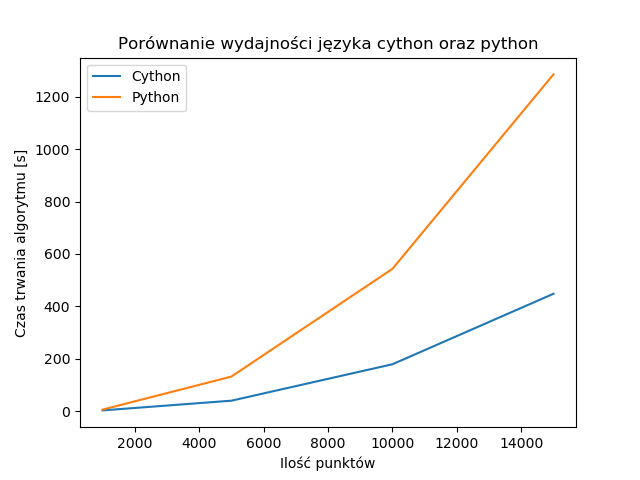
\includegraphics[scale=0.48]{pythonvscython.png}
  \caption{Porównanie czasu algorytmu dla cython oraz python.}   
  \label{fig:pytcytpic}
\end{figure}
\begin{table}[H]
\begin{center}
\caption{\label{tab:cythonVsPython}Porównanie czasu trwania algorytmu dla cython oraz python.}
\centerline{
\begin{tabular}{ |c|c|c| }
 \hline
 { Liczba punktów} & { Czas cython}& { Czas python}\\ 
  \hline
   {\small 1000 pkt} & {\small 2.97 s} & {\small 6 s}  \\  
  \hline 
     {\small 5000 pkt} & {\small 40 s}& {\small 132 s}   \\  
  \hline
   {\small  10000 pkt} & {\small 179 s}& {\small  543 s}   \\  
  \hline
 {\small  15000 pkt} & {\small 448 s}& {\small  1285 s}   \\  
  \hline
\end{tabular}
}
\end{center}
\end{table}



Na wykresie \ref{fig:pytcytpic} oraz w tabeli \ref{tab:cythonVsPython} można zauważyć, że wstępna kompilacja kodu nie tylko wpłynęła procentowo na wydajność algorytmu. Sprawiła ona, iż tempo wzrostu złożoności obliczeniowej w zależności od ilości punktów również się zmniejszyło. Dzięki temu możliwe jest wykonanie triangulacji jeszcze większej ilości punktów. Zmniejszenie tempa wzrostu ma związek z optymalizacją pętli iteracyjnych w języku cython. Wraz ze wzrostem ilości punktów poddanych triangulacji, rośnie również ilość iteracji pętli. W języku python pętle wykonywane są wolniej niż w cython, dlatego też przyrost czasu obliczeniowego jest znacznie bardziej dostrzegalny.

Następnym elementem który wpłynął pozytywnie na optymalizację czasu działania programu jest zmiana biblioteki. Dotychczas do obliczania wyznacznika macierzy używana była funkcja z biblioteki NumPy. Jest to biblioteka typu open-source. Dostęp do niej jest darmowy, a aktualizować ją może każdy kto zostanie zaakceptowany przez społeczność. Dzięki pracy dużej liczby ludzi kod jest zoptymalizowany oraz uniwersalny. Funkcje dostępne w NumPy mają bardzo dużą wydajność pod względem pamięci i zasobów obliczeniowych. Biblioteka zawiera wiele różnych modułów począwszy od algebry liniowej, po równania różniczkowe oraz obliczenia na liczbach zespolonych. Z testów przeprowadzonych na programie do triangulacji wynika, że do obliczeń macierzowych najlepiej jednak się biblioteka SciPy. Ona też jest zbiorem programów typu open-source. Korzysta ona po części z NumPy jako struktury do przechowywania danych obliczeniowych. Obie biblioteki zawierają podobne funkcje, lecz do zastosowań projektowych wybrana została ta druga. Porównanie pracy programu, przy zastosowaniu funkcji z biblioteki NumPy oraz SciPy do obliczeń macierzowych zostało przedstawione w tabeli \ref{tab:numpyVsScipy}.
\begin{table}[H]
\begin{center}
\caption{\label{tab:numpyVsScipy}Porównanie czasu trwania algorytmu przy obliczaniu macierzy przez NumPy oraz SciPy.}
\centerline{
\begin{tabular}{ |c|c|c| }
 \hline
 { \small Liczba punktów} & { \small Czas SciPy}& {\small Czas NumPy}\\ 
  \hline
   {\small 1000 pkt} & {\small 2.97 s} & {\small 2.48 s}  \\  
  \hline 
     {\small 5000 pkt} & {\small 40 s}& {\small 36 s}   \\  
  \hline
   {\small  10000 pkt} & {\small 179 s}& {\small  231 s}   \\  
  \hline
 {\small  15000 pkt} & {\small 448 s}& {\small  486 s}   \\  
  \hline
\end{tabular}
}
\end{center}
\end{table}
W powyższej tabeli został przedstawiony wpływ użycia różnych bibliotek na ostateczny czas trwania algorytmu triangulacji Delaunay'a. Dla mniejszej ilości punktów, biblioteka NumPy jest wydajniejsza. Jednak przy wzroście punktów, biblioteka SciPy osiągnęła lepsze wyniki, dlatego została wybrana jako docelowa metoda przeprowadzania obliczeń macierzowych.  

Kolejnym aspektem algorytmu wymagającym znacznej mocy obliczeniowej jest badanie styczności czworościanów. W algorytmie, z każdej ściany ostrosłupa niestykającej się z inną ścianą jest budowany jest dodatkowy czworościan. W jego skład wchodzą trzy wierzchołki początkowej ściany oraz dodatkowy punkt triangulacyjny. Należy, więc znaleźć te ściany algorytmu, które nie stykają się z pozostałymi. Jest to zadanie wymagające dwóch pętli iteracyjnych i wykonywane jest dla każdego dodatkowego punktu. W przypadku autorskiego programu, zostało zastosowane kryterium przynależności zbiorów. Tablica ścian została utworzona poprzez kombinację 4 różnych wierzchołków. Dla każdego z pozostałych czworościanów sprawdzane jest czy którekolwiek z trzech wierzchołków znajdują się w zbiorze ścian początkowego ostrosłupa. Jeśli tak, to ściana ta jest dodawana do zbioru zajętych ścian i proces jest kontynuowany do momentu wyczerpania pozostałych ostrosłupów lub ścian. Zadanie to nie jest trywialne z punktu widzenia struktury danych. Matematyczne podstawy jego funkcjonowania nie są złożone, jednakże opis programowy tak. Wymagana jest struktura, która umożliwia przechowywanie nieuporządkowanej sieci wierzchołków. Dzieje się tak ze względu na to, że punkty mogą tworzyć ścianę w różnej kolejności, więc porządek ich występowania w danej ścianie może być różny dla dwóch osobnych ostrosłupów. Zostały sprawdzone dwie metody odnajdywania sąsiadujących ścian.
\newline \indent Pierwsza metoda zakładała iterację przez wszystkie wierzchołki początkowego oraz aktualnego czworościanu. Dzięki temu można było sprawdzić ile z nich występuje w obu tych zbiorach. To zadanie wymagało dużo czasu obliczeniowego, ponieważ korzystało z trzech pętli iteracyjnych. Pierwsza odpowiadała za wybór sąsiedniego ostrosłupa, druga za wybór ściany do sprawdzenia w aktualnym czworościanie, a trzecia za wybór ściany w drugim ostrosłupie.
\newline \indent Drugą metodą, która była możliwa dzięki zastosowaniu języka python były operacje na zbiorach. Struktura danych set() umożliwia przechowywanie nieuporządkowanych zbiorów danych i dokonywanie na nich operacji. Na potrzeby algorytmu triangulacyjnego zastosowano iloczyn dwóch zbiorów.
\begin{equation}
    \begin{aligned}
    \begin{cases}
    &V_{a}={v_{a1},v_{a2},v_{a3},v_{a4}}\\
    &V_{b}={v_{b1},v_{b2},v_{b3},v_{b4}}\\
    &S_{a}=\binom{V_{a}}{3}\\
    &S_{b}=\binom{V_{b}}{3}\\
    &W=V_{a} \cap V_{b}\\
    &S_{bi} 	\subset S_{a} \Leftrightarrow |W|=3\\
    &S_{f}=S_{a}/S_{bi}
    \end{cases}
    \end{aligned}
\end{equation}
Ostrosłupy A oraz B są opisane wierzchołkami znajdującymi się odpowiednio w zbiorach $V_{a}$ i $V_{b}$. Ściany obydwóch ostrosłupów znajdują się w zbiorach $S_{a}$ oraz $S_{b}$. Wspólne wierzchołki ostrosłupów stanowią zbiór $W$, zaś zbiór $S_{f}$ zawiera ściany wolne niestykające się z pozostałymi ostrosłupami.
\newline \indent Z powyższych równań widać, że jeśli moc zbioru będącego iloczynem zbiorów wierzchołków ostrosłupów będzie równa 3, to obie te figury będą posiadały wspólną ścianę. Należy ją wtedy dodać do zbioru współdzielonych ścian. Operacja zostanie powtórzona dla wszystkich pozostałych ostrosłupów. Ze ścian wolnych które pozostaną, zostaną zbudowane nowe ostrosłupy.
\newline \indent Na sam koniec, ze zbioru ostrosłupów triangulacyjnych należy usunąć te, które współdzielą krawędzi z początkowym super-ostrosłupem. Operację można szybko przeprowadzić, ponieważ znane są współrzędne wierzchołków początkowego czworościanu. 
\newline \indent Powyższe operacje przedstawiają algorytm triangulacji Delaunay'a, dzięki któremu uzyskiwane są ostrosłupy. Do generacji meshu potrzebna jest jeszcze dodatkowa rzecz. Mianowicie, muszą zostać utworzone poszczególne ściany tych ostrosłupów. Są one generowane poprzez kombinację wierzchołków ostrosłupa. Następnie, współrzędne wierzchołków muszą zostać przekształcone na odpowiadające im indeksy w zbiorze punktów. W celu optymalizacji algorytmu każdy punkt posiada czwartą współrzędną. Jest nią indeks na którym znajduje się punkt w ogólnym zbiorze punktów. Umożliwia to w końcowym etapie szybkie przekształcenie ścian bryły do postaci indeksów.
\newline \indent Ostatnim etapem programu jest zapis utworzonego w ten sposób meshu do pliku. Wykonywane jest to za pomocą biblioteki Trimesh. Jako parametr podawany jest tam zbiór ścian ostrosłupa. Kolejnymi parametrami są kolory wierzchołków oraz ich współrzędne. Tak wygenerowany plik może zostać wyeksportowany i otwarty w programie Blender. Poprzez wykorzystanie programu Blender, możliwe jest dokonywanie różnych operacji na wygenerowanym modelu. Aplikacja zawiera szereg funkcji, umożliwiających wykonywanie różnych przekształceń na obiekcie. Dodatkowo można w sposób ręczny usunąć błędnie wygenerowane trójkąty triangulacyjne, udoskonalając w ten sposób przygotowany model trójwymiarowy.

\section{Przedstawienie wyników oraz omówienie}
Powyższe algorytmy miały na celu jak najdokładniej odwzorować obiekt na podstawie danych z kamery głębi. W poniższej sekcji omówione zostaną wyniki użytych metod. Ukazane zostaną modele utworzone poprzez wykorzystanie algorytmu BPA oraz triangulacji Delaunay'a. Przedstawiona zostanie dokładność odwzorowania powierzchni oraz procentowa zawartość dziur. W celu testów wykonano dwa skany przedmiotów. Dokonano przekształcenia na model 3D jabłka oraz pudełka. Oba te przedmioty mają swoje barwy które również zostały oddane w modelach.
\subsection{Algorytm BPA}
Dla algorytmu toczącej się kuli dokonano pomiaru wpływu promienia na ostateczny wygląd modelu. Dla ukazania rzeczywistego wyglądu modeli zostały dodane chmury punktów. Na rysunku \ref{fig:pointCloudFig} znajdują się punkty z nałożoną teksturą dla modeli jabłka oraz pudełka.
\begin{figure}[H]
\centering
    \begin{minipage}[b]{0.45\linewidth}
        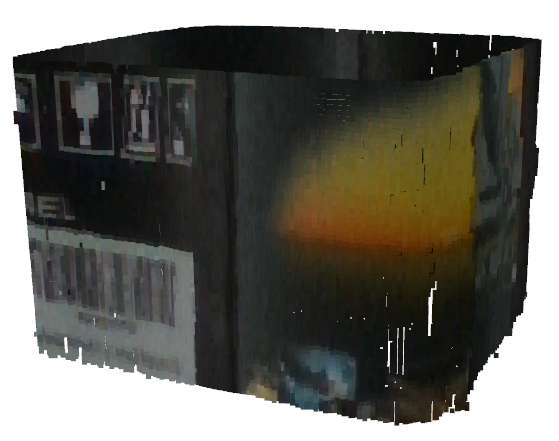
\includegraphics[scale=0.6]{pudelkoPointcloud.PNG}
    \end{minipage}
\quad
    \begin{minipage}[b]{0.45\linewidth}
        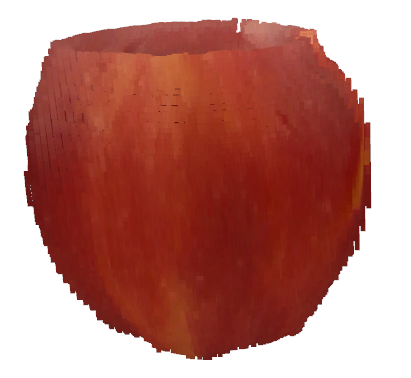
\includegraphics[scale=0.6]{jablkoPointcloud.PNG}

    \end{minipage}
\caption{Chmury punktów pudełka oraz jabłka.}
\label{fig:pointCloudFig}
\end{figure}

W celu sprawdzenia wpływu długości promienia kuli na ostateczny wygląd modelu dokonano porównania. Na rysunkach \ref{fig:appleComparison1},\ref{fig:appleComparison2},\ref{fig:boxComparison1} i \ref{fig:boxComparison2} znajdują się modele jabłka oraz pudełka na które został nałożony mesh korzystając z metody BPA. Dla każdego z nich sprawdzono wartość promienia R równą odpowiednio 2,5,7,10 razy średnia odległość pomiędzy punktami. Dla lepszego porównania zdjęcia modeli robiono pod podobnym kątem.


\begin{figure}[H]
\centering
    \begin{minipage}[b]{0.45\linewidth}
        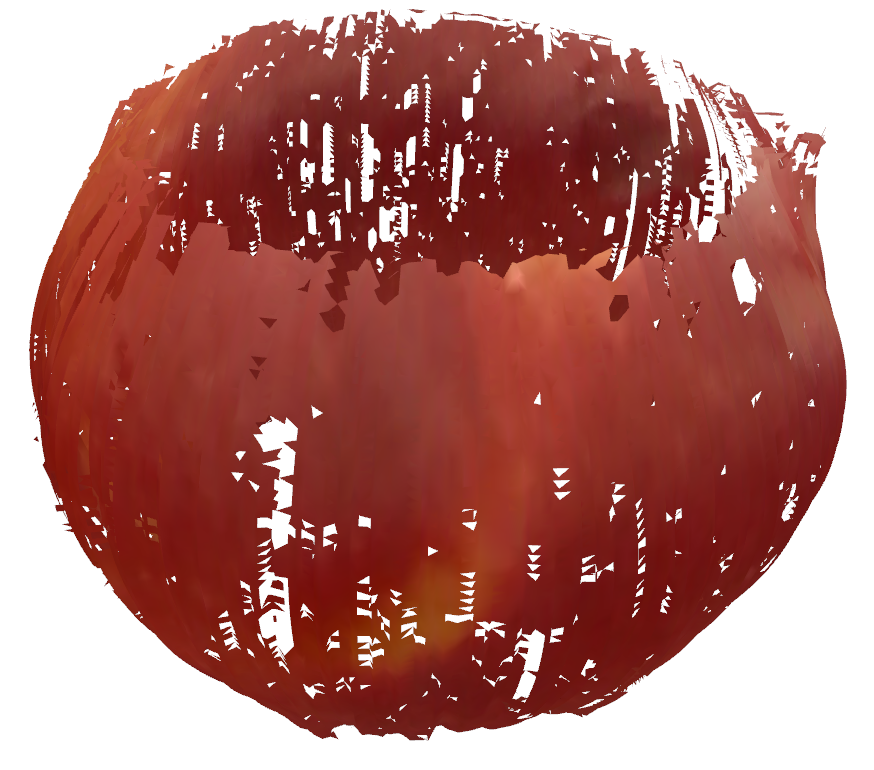
\includegraphics[scale=0.3]{bpaApple2x.PNG}
    \end{minipage}
\quad
    \begin{minipage}[b]{0.45\linewidth}
        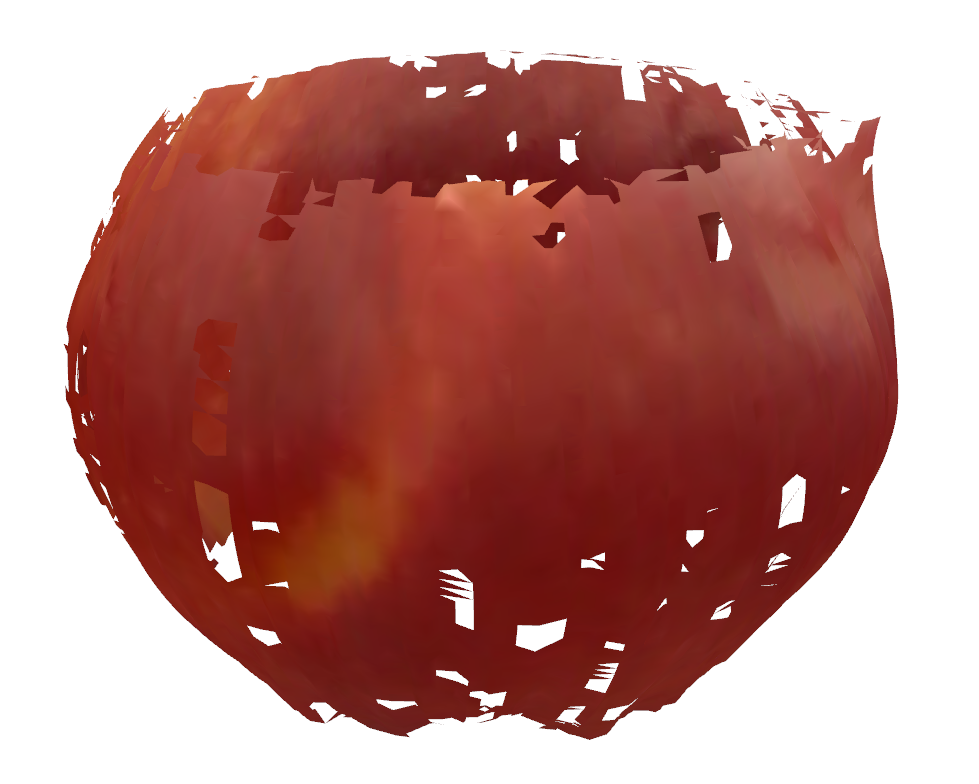
\includegraphics[scale=0.3]{bpaApple5x.PNG}
    \end{minipage}
\caption{Mesh BPA dla R=2$D_{mean}$ T=1.41 s oraz R=5$D_{mean}$ T=78 s .}
\label{fig:appleComparison1}
\end{figure}

\begin{figure}[H]
\centering
    \begin{minipage}[b]{0.45\linewidth}
        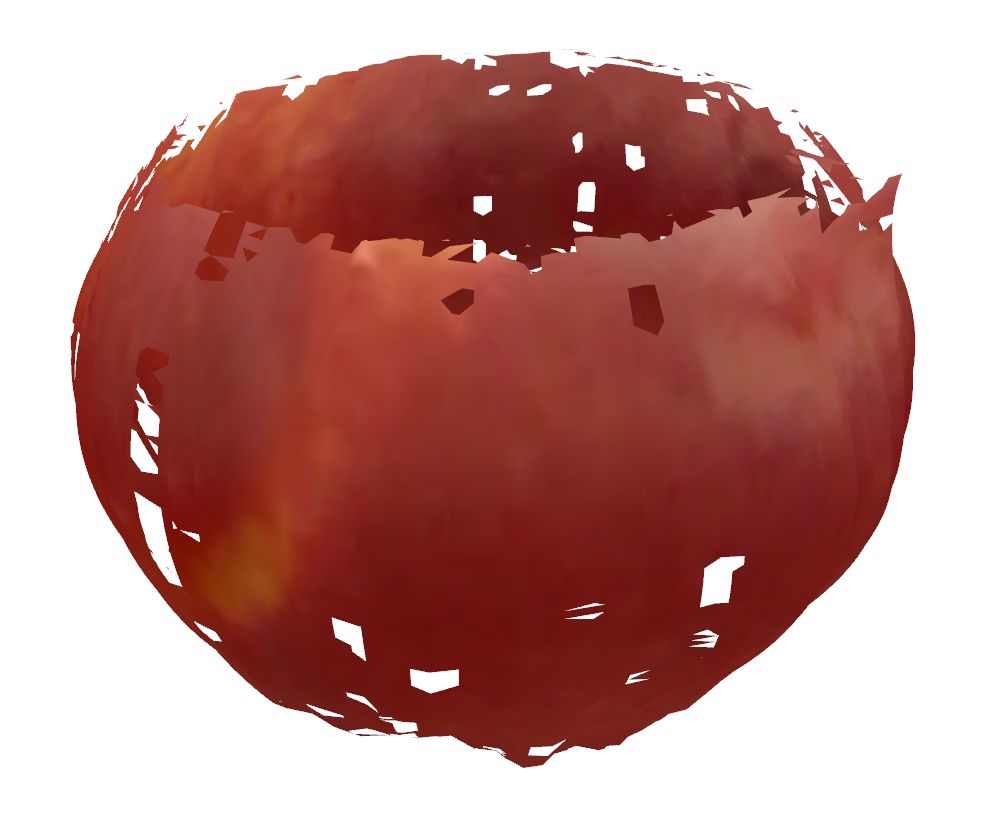
\includegraphics[scale=0.3]{bpaApple7x.PNG}
    \end{minipage}
\quad
    \begin{minipage}[b]{0.45\linewidth}
        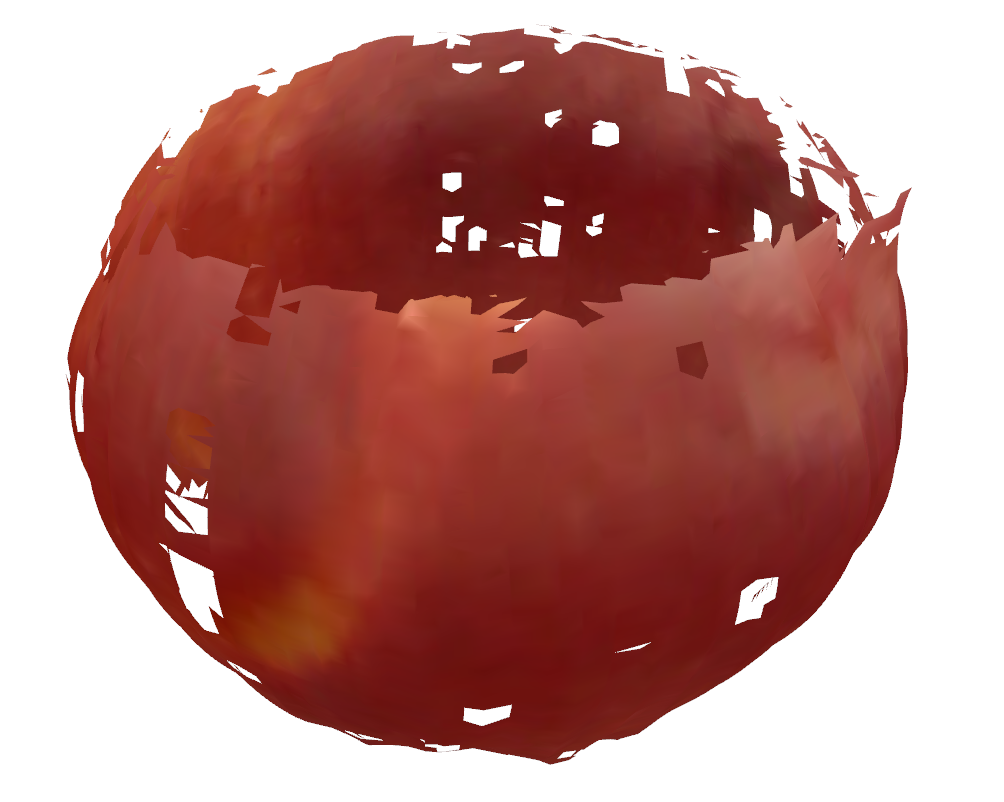
\includegraphics[scale=0.3]{bpaApple10x.PNG}
    \end{minipage}
\caption{Mesh BPA dla R=7$D_{mean}$ T=331 s oraz R=10$D_{mean}$ T=1532 s .}
\label{fig:appleComparison2}
\end{figure}

\begin{figure}[H]
\centering
    \begin{minipage}[b]{0.45\linewidth}
        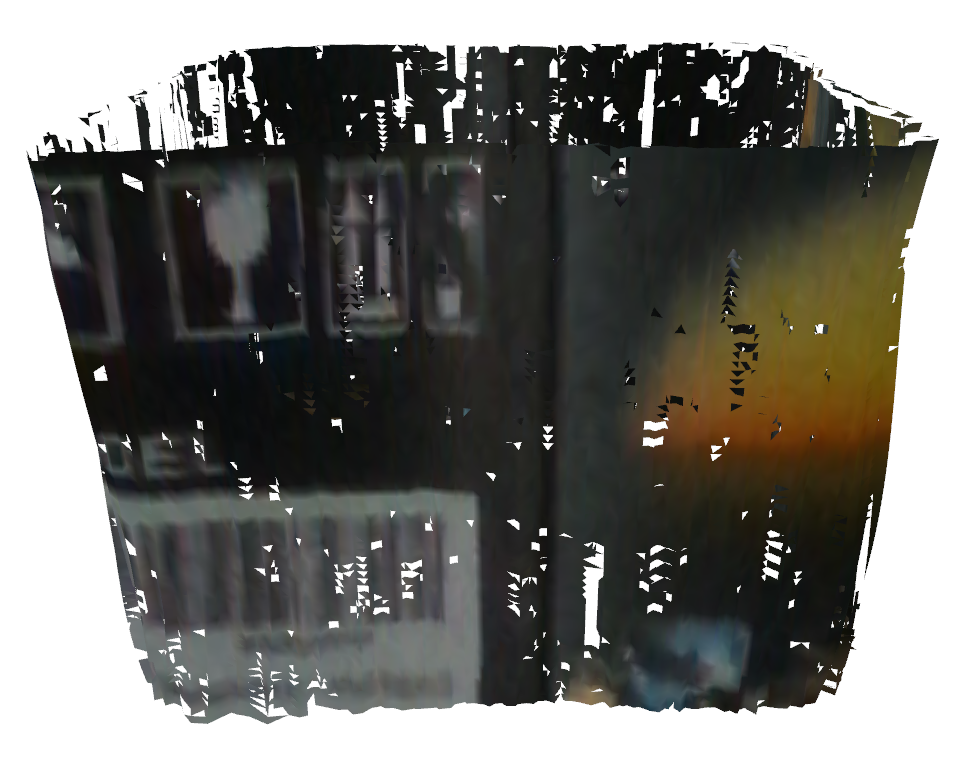
\includegraphics[scale=0.3]{bpaBox2x.PNG}
    \end{minipage}
\quad
    \begin{minipage}[b]{0.45\linewidth}
        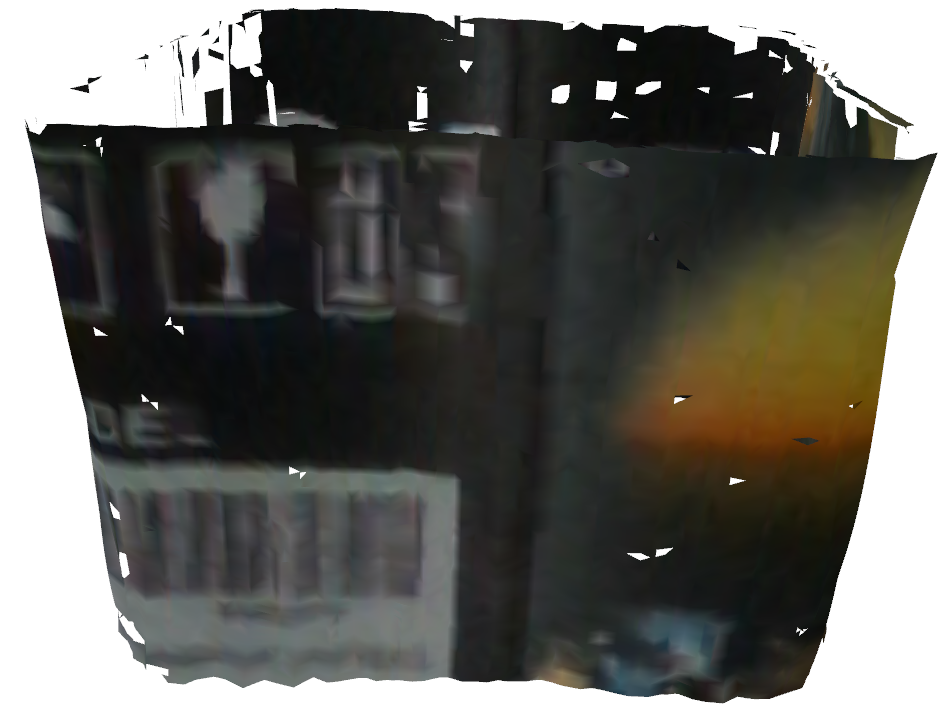
\includegraphics[scale=0.3]{bpaBox5x.PNG}
    \end{minipage}
\caption{Mesh BPA dla R=2$D_{mean}$ T=1.04 s oraz R=5$D_{mean}$ T=53 s .}
\label{fig:boxComparison1}
\end{figure}

\begin{figure}[H]
\centering
    \begin{minipage}[b]{0.45\linewidth}
        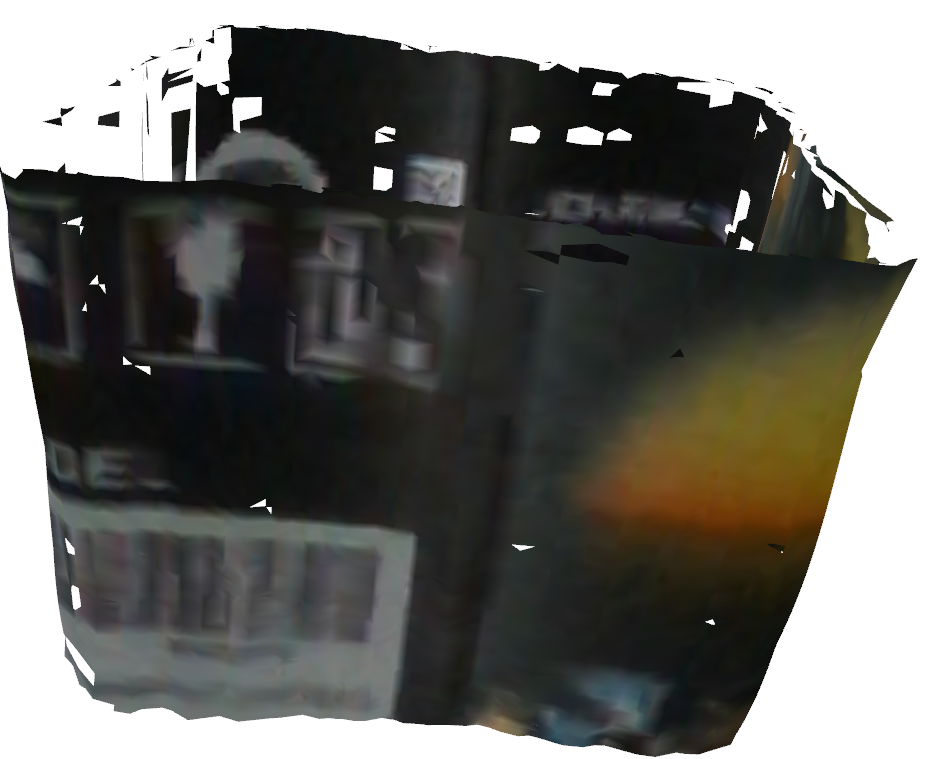
\includegraphics[scale=0.3]{bpaBox7x.PNG}
    \end{minipage}
\quad
    \begin{minipage}[b]{0.45\linewidth}
        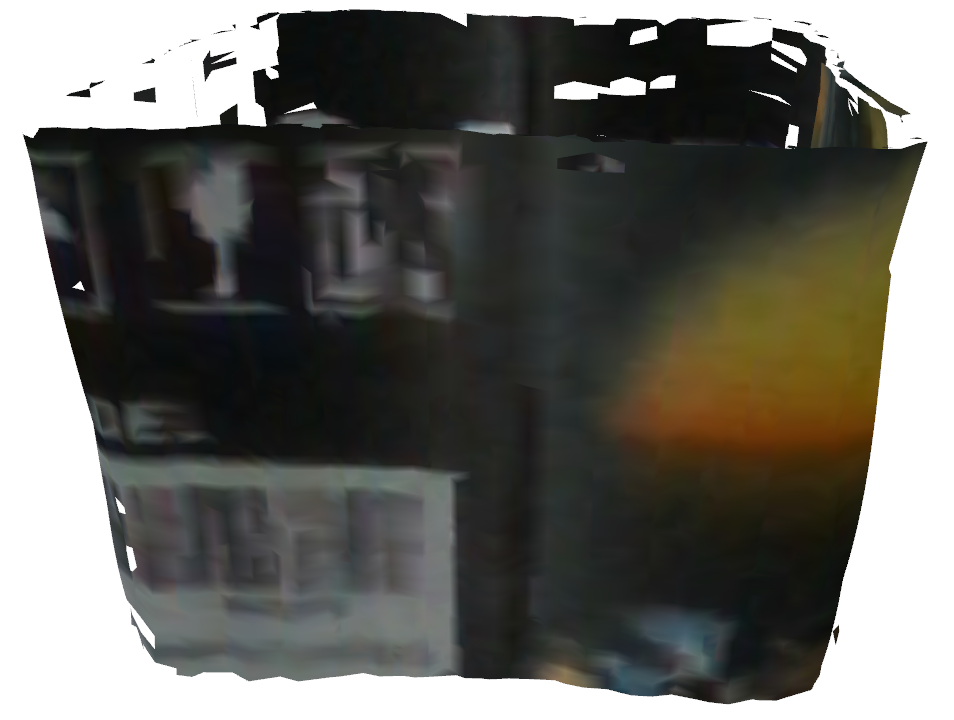
\includegraphics[scale=0.3]{bpaBox10x.PNG}
    \end{minipage}
\caption{Mesh BPA dla R=7$D_{mean}$ T=233 s oraz R=10$D_{mean}$ T=1071 s .}
\label{fig:boxComparison2}
\end{figure}
Na powyższym zestawieniu widać, że wygląd chmury punktów znacząco różni się od gotowego meshu. W modelu jest wiele luk, które należy zakryć. Dokonać tego można przez odpowiednie dobranie promienia kuli. Znaczący wpływ na luki ma nierównomierna gęstość rozłożenia punktów w chmurze. Dla długości promienia równej dwukrotnej średniej odległości punktów, na rysunku \ref{fig:appleComparison1} oraz \ref{fig:boxComparison1} widać znaczny ich odsetek. Zwiększenie promienia do 5 znacznie poprawia wypełnienie. Po tym etapie, dalsze powiększanie promienia wpływa nieznacznie na ostateczny wygląd.

Przy zwiększaniu promienia rośnie również czas obliczeniowy. Powodem tego jest większa ilość punktów w sąsiedztwie kuli. Dla każdego jej przesunięcia wymagane jest wyznaczenie sąsiadów z odległości 2R, co przy większym promieniu oznacza znaczną ilość punktów. Dla małej długości promienia czas obliczeń jest stosunkowo dobry. Algorytm zajmuje około 50 sekund. Można jednak zauważyć gwałtowną tendencję wzrostową. Zwiększenie o mniej niż 50 \% długości promienia, sprawia , że długość obliczeń wzrasta pięciokrotnie. W celu najlepszych wyników zarówno czasowych jak i wyglądu modeli należy empirycznie dobrać promień. Z obserwacji wynika, że promień równy trzykrotności średniej odległości punktów daje dobre rezultaty. Został to też potwierdzone w pracach naukowych \cite{mittleman1999ball}. Z ich badań wynika, że średnio w sąsiedztwie kierunku toczenia się kuli powinno znajdować się 20 punktów. Przy R=3$D_{mean}$ wzdłuż oraz wokół promienia znajduje się 17 punktów. Oznacza to, że empirycznie dobrany promień jest dobrym punktem startowym do poszukiwań.

\subsection{Algorytm Delaunay}
W autorskim programie została w całości zaimplementowana metoda triangulacji Delauny'a. W poniższej sekcji opisane zostaną wyniki pomiarów, wygenerowane modele oraz ich udoskonalenia w programie Blender. Na rysunku \ref{fig:delaBoxApple} ukazane zostały triangulacje Delaunay'a dla chmur punktów jabłka oraz pudełka.
\begin{figure}[H]
\centering
    \begin{minipage}[b]{0.45\linewidth}
        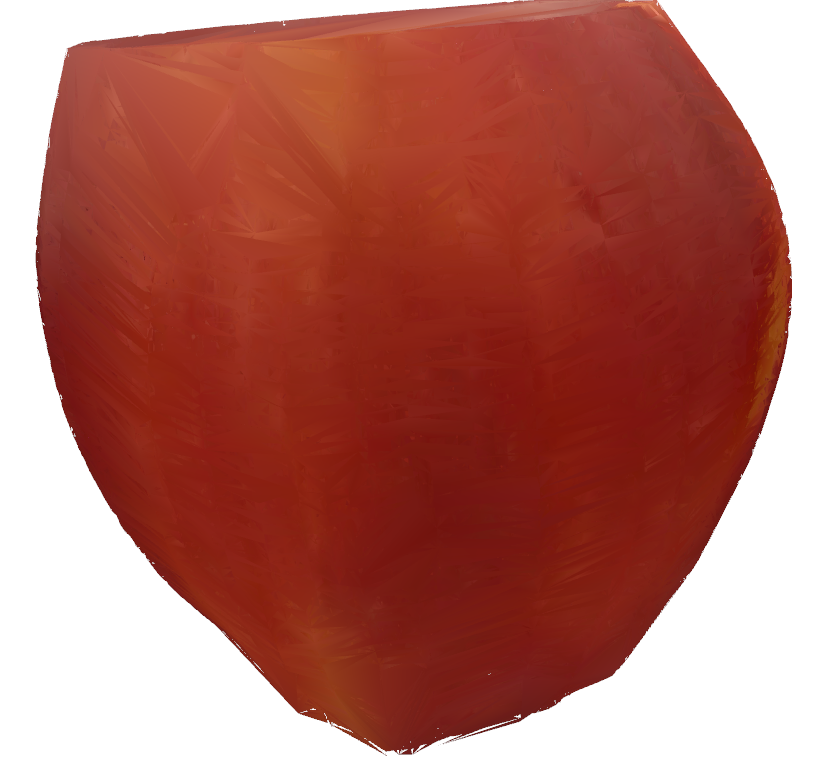
\includegraphics[scale=0.3]{jablkoDelNowe.PNG}
    \end{minipage}
\quad
    \begin{minipage}[b]{0.45\linewidth}
        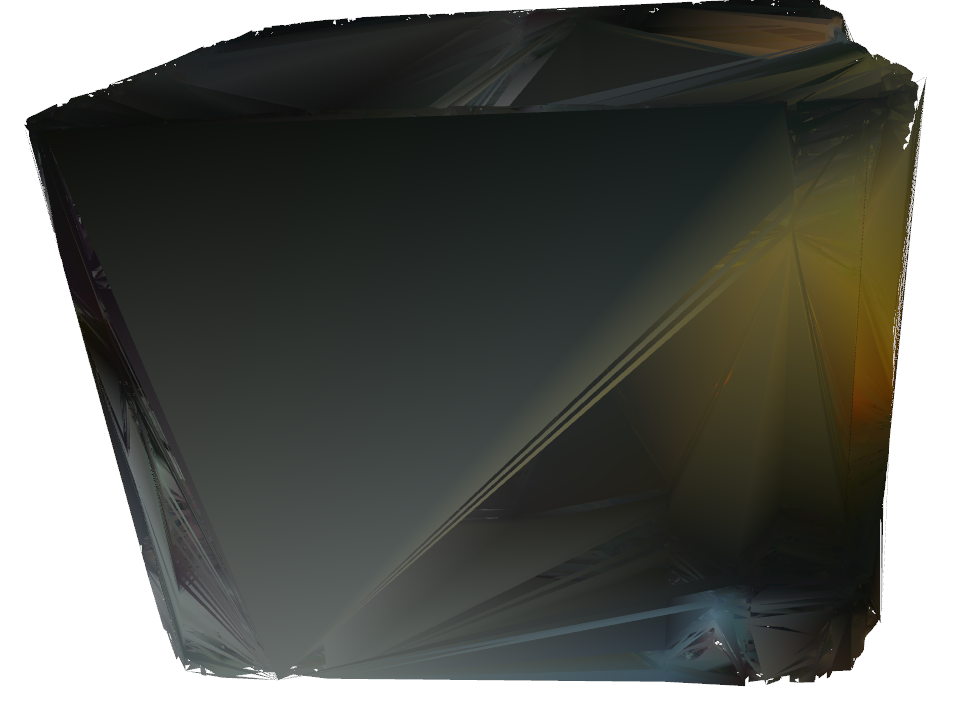
\includegraphics[scale=0.3]{delaunayBox.PNG}
    \end{minipage}
\caption{Mesh Delaunay dla jabłka oraz pudełka.}
\label{fig:delaBoxApple}
\end{figure}
Na rysunku powyżej można zauważyć najważniejszą różnicę algorytmu BPA od triangulacji Delauny'a. W przypadku pierwszego, wygenerowane modele zawsze zawierały pewien odsetek dziur. Jednakże, ze względu na istotę działania, modele uzyskane dzięki wykorzystaniu algorytmu Bowyera-Watsona ich nie zawierają. Wynika to z faktu, iż do poprawnego funkcjonowania tej metody, z każdej trójki punktów musi zostać utworzony trójkąt. Dzięki temu z każdego punktu w chmurze tworzona jest ściana ostrosłupa. Ponadto korzystając z danej metody, zostają również uzupełnione luki wynikające ze sposobu pomiaru. Akwizycja danych następuje z boku obiektu, dlatego nie istnieją dane o wierzchniej powierzchni modeli. Triangulacja Delaunay'a rozwiązuje ten problem, ponieważ graniczne punkty są łączone z pozostałymi na drugiej ścianie, tworząc w ten sposób dotychczas nieistniejącą ścianę. Kolory ścian wyznaczane są na podstawie wierzchołków trójkąta. 

Mankamentem tej metody jest fakt, że często ściany występujące w modelu są duże. Oznacza to, że niekiedy część krawędzi obiektu może zostać przysłonięta przez zbudowaną ścianę. Taka sytuacja została zaprezentowana na rysunku \ref{fig:delaBoxApple} w przypadku modelu pudełka. Kolory zostały wiernie oddane, jednak część z nich na siebie nachodzi, przysłaniając w ten sposób pozostałe. W przypadku jabłka ten problem nie występuje.

Wykorzystując program do obróbki modeli Blender, można dodatkowo wygładzić ściany z ostrych krawędzi powstałych w skutek triangulacji. Program zawiera szereg funkcji wpływających na wygląd gotowego meshy, zmieniając sposób w jaki światło się od nich odbija. Na rysunku \ref{fig:blenderDela} przedstawione zostały modele poddane obróbkom.

\begin{figure}[H]
\centering
    \begin{minipage}[b]{0.45\linewidth}
        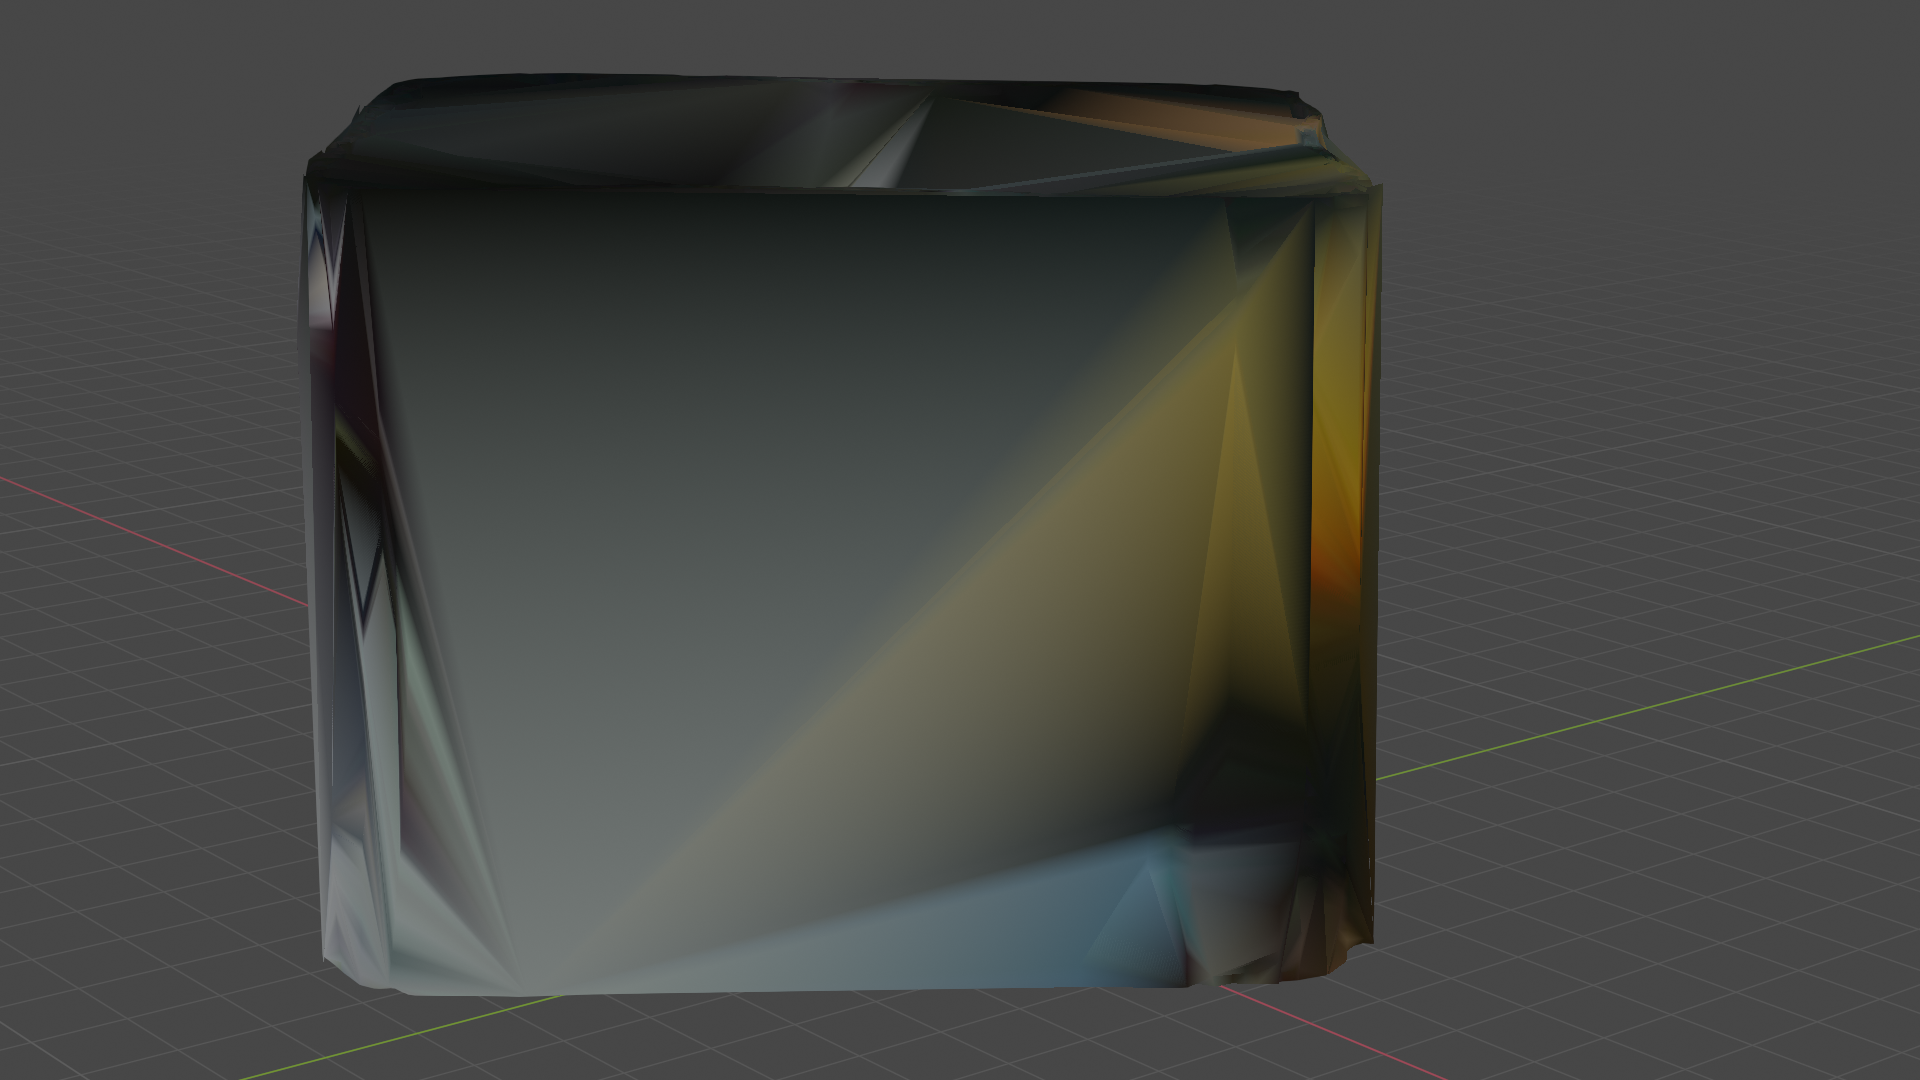
\includegraphics[scale=0.12]{delaBlendBoxgladkie.PNG}
    \end{minipage}
\quad
    \begin{minipage}[b]{0.45\linewidth}
        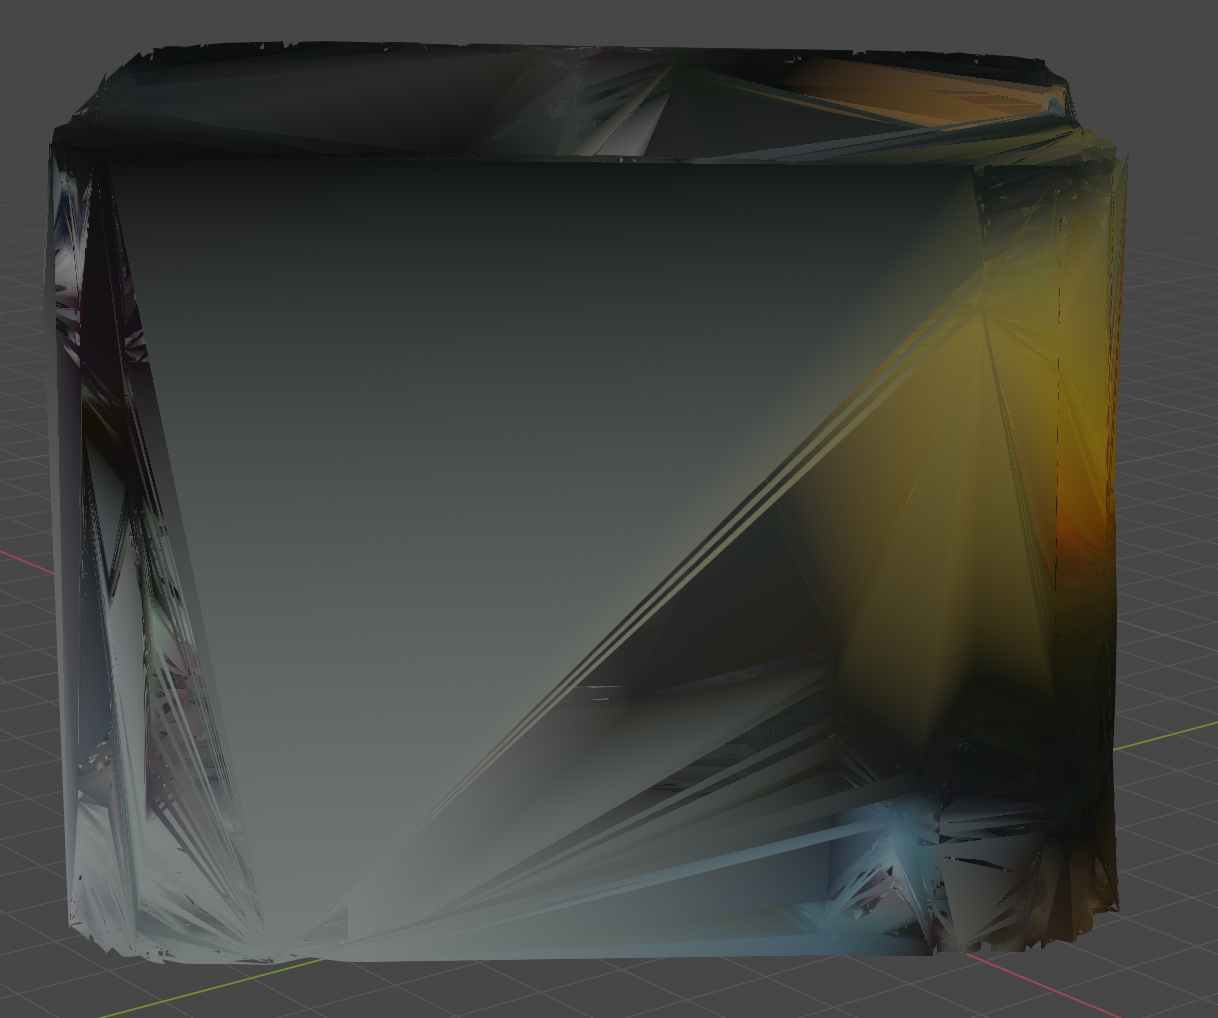
\includegraphics[scale=0.12]{delaBlendBoxNiegladkie.png}
    \end{minipage}
\caption{Mesh Delaunay dla pudełka przed i po wygładzaniu w programie Blender.}
\label{fig:blenderDela}
\end{figure}
Na powyższym rysunku przedstawiono modele przekształcone za pomocą programu Blender. Zastosowano funkcję flat do wyrównania poziomu cieni wokół wystających krawędzi, dzięki czemu stają się one mniej widoczne. Po lewej stronie wprowadzono funkcję, zakrywającą tylne krawędzie. Wykorzystując te metodę można uzyskać gładkie boki sześcianu, co wpływa pozytywnie na wygląd modelu. Część krawędzi przekształcono za pomocą edycji wierzchołków. Jest to funkcja pozwalająca na wygładzanie wystających wierzchołków trójkątów triangulacyjnych. Możliwe jest też podnoszenie tych, które leżą zbyt nisko, dzięki czemu ściany mają naturalny kształt. 
\begin{figure}[H]
  \centering
  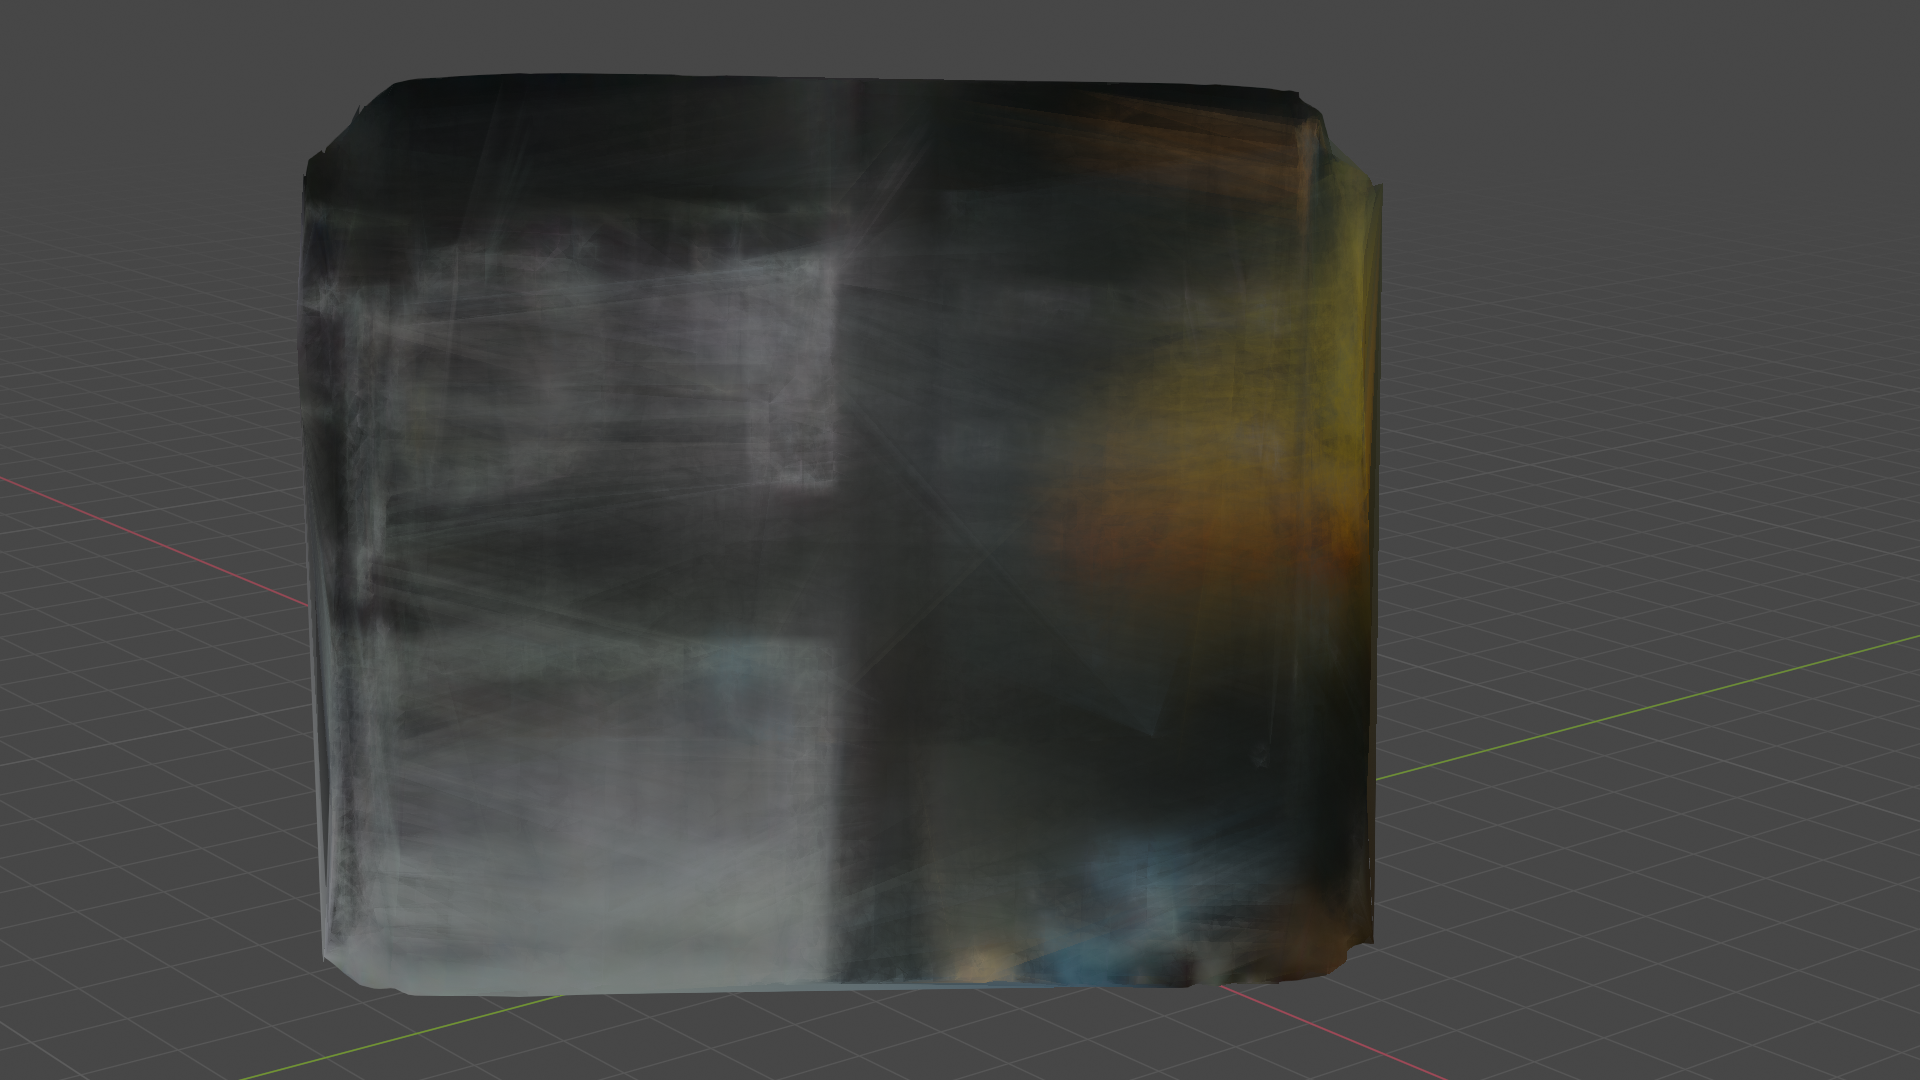
\includegraphics[scale=0.2]{delaBlendBoxXray.png}
  \caption{Ukryte ściany pudełka widoczne w programie Blender.}   
  \label{fig:pytcytpic}
\end{figure}
Na rysunku powyżej zastosowano funkcję Xray. Pozwala ona na wyświetlenie dolnych warstw obiektu. Wykorzystując to przekształcenie, można zauważyć, że triangulacja Delaunay'a działa poprawnie. Ściany które dotychczas były ukryte, ukazują faktyczną teksturę obiektu która pokrywa się z tą wygenerowaną przez chmurę punktów.

Ostatecznie wybrano triangulację Delaunay'a do przeprowadzania generacji meshu. Pomimo wad takich jak przykrywanie wierzchnich warstw powierzchni przez trójkąty daje ona dobre rezultaty. Ściany modelu nie zawierają dziur. Poprzez wykorzystanie tego algorytmu generowane zostają też ściany, które w przypadku BPA nie mogły zostać utworzone. Taka sytuacja jest dla dolnej oraz górnej ściany prostopadłościanu oraz jabłka. Delaunay generując trójkąty łączy również przeciwległe ściany zakrywając tym samym obszary nieobjęte przez chmurę punktów. Poprzez zastosowanie danej metody uzyskuje się zawsze taki sam rezultat. Wygląd modelu nie zależy od nastaw parametru, tak jak miało to miejsce w przypadku BPA. Usprawnia to proces konwersji fizycznych obiektów do postaci 3D,a dzięki programowi Blender można dodatkowo usunąć niepotrzebne trójkąty zakrywające pozostałe ściany.




\chapter{Zako{\'n}czenie}
% W poniższym rozdziale omówione zostaną wyniki przeprowadzonych badań. Dokonane zostanie porównanie algorytmu BPA z gotowej biblioteki, autorskiej implementacji algorytmu Delaunay'a oraz gotowych meshy dostępnych w innych pracach naukowych. Ukazane zostaną możliwości poprawy i udoskonalenia programu oraz niedoskonałości, które w przyszłości powinny zostać zmodernizowane. 

% \section{Podsumowanie}
Tematem pracy jest zbudowanie skanera 3D oraz wyeksportowanie gotowych modeli do programu Blender. Dane zadanie zostało wykonane pomyślnie. Przeprowadzono analizę dostępnych metod oraz teoretyczną analizę algorytmów. Dokonano szeregu optymalizacji, wpływających na zwiększenie wydajności autorskiego programu. Postawiony problem był złożony, a na ostateczny wygląd modelu wpływał szereg czynników. W poniższej sekcji przytoczone zostaną najważniejsze z nich.
\subsection{Budowa skanera}
W celu odpowiedniej akwizycji danych należało skonstruować skaner 3D. Po wielu testach wyznaczono jego poprawny schemat. Istotnym czynnikiem była platforma poruszająca się ze stałą prędkością kątową. Bez niej zadanie byłoby niemożliwe do zrealizowania. Odpowiedni dobór kamery trójwymiarowej również wywarł wpływ na jakość modeli. W przypadku początkowej kamery Orbbec Astra Mini rozdzielczość zdjęć była niska, wynosiła maksymalnie 640x480 pikseli. Z kolei rozdzielczość Intel RealSense D435i jest prawie dwukrotnie wyższa. Rozdzielczość kamery znacznie wpływa na jakość ostatecznego modelu, im jest ona większa, tym chmura punktów jest gęstsza. W rezultacie powoduje to bardziej dokładne odwzorowanie powierzchni obiektu. Poprzez zastosowanie wysokiej rozdzielczości kamery oraz dużej liczbie klatek na sekundę, rozmiar zapisywanych danych jest obfity. Film trwający 58 sekund, zawierający dane o głębi oraz kolorze obiektu dla rozdzielczości 848x 640, zajmuje około 1.7 GB i 2.3GB dla odpowiednio 15 klatek na sekundę oraz 30 klatek na sekundę. Kamera podłączona jest do komputera poprzez gniazdo USB 3.2, niższy standard transmisji danych nie byłby w stanie przesłać takiej ilości informacji. Protokół USB 3.2 jest jednak wciąż zbyt niski, by przesyłać nagranie 1280x720 dla 90 klatek. Prawdopodobnie podłączenie kamery bezpośrednio pod złącze PCI-e byłoby w stanie przesłać taki rozmiar danych. Z danych producenta wynika, że dla rozdzielczości 848x480 koloru oraz głębi dla 90 klatek, rozmiar przesyłanych danych to 1172 Mbps.

Kalibracja kamery jest równie ważna co budowa skanera. By otrzymać najlepsze rezultaty należy odpowiednio nastawić moc emitera, ekspozycję oraz odpowiednio skalować dane głębi by pokrywały się one z rzeczywistymi wartościami. Dzięki wykorzystaniu dedykowanego oprogramowania Intel RealSense Viewer oraz Intel RealSense Depth Quality Tool możliwy był podgląd obrazu z kamery w czasie rzeczywistym. Zmniejszyło to czas kalibracji, ponieważ rezultaty były widoczne natychmiast po zatwierdzeniu. Depth Quality Tool pozwala na sprawdzenie, jak wybrane nastawy wpływają na ilość dziur w nagraniu. Im jest ich mniej, tym dane będą mniej przekłamane, a model będzie wierniej oddawał rzeczywisty obiekt.
\subsection{Akwizycja oraz obróbka danych}
Kolejnym istotnym czynnikiem wpływającym na ostateczny wygląd modelu jest wybrana metoda akwizycji danych. Przeprowadzono analizę chmur punktów powstałych poprzez zastosowanie dwóch metod przetwarzania danych. W metodzie skanera liniowego pod uwagę brana tylko jedna kolumna obrazu, zaś w metodzie światła strukturalnego użyto danych głębi pochodzących z całej klatki. Po analizie otrzymanych wyników z obu metod wybrano metodę skanera liniowego, ze względu na lepszy wygląd ostatecznego modelu. Dzięki jej wykorzystaniu przekształcenia trygonometryczne są prostsze, a czas trwania obliczeń jest znacznie mniejszy. Po uzyskaniu danych z kamery RGBD należy je odpowiednio przetworzyć. Bezpośrednie pomiary głębi zawierają przekłamane punkty, które należy odnaleźć. W przeciwnym wypadku wpłyną one na wygląd modelu po triangulacji Delaunay'a, ponieważ zostaną utworzone z nich zbyt duże trójkąty. Często przekłamane punkty mają wartość odpowiadającą maksymalnej rozdzielczości głębi kamery, więc punkty znajdą się wiele metrów dalej niż rzeczywisty model. To znacząco wpływa na pogorszenie jakości gotowego modelu. W celu uniknięcia tych błędów należy odnaleźć przekłamane punkty. W programie dokonano tego przez liczenie średniej odległości punktów od środka układu współrzędnych. Jeśli odległość przekłamanego punktu będzie o wiele większa niż średnia, to zostanie on oznaczony flagą. Oznaczone w ten sposób punkty, poddane zostaną interpolacji w celu wyznaczenia poprawnej ich wartości.
\newline \indent Po przeprowadzeniu testów różnych metod interpolacji, wybrana została interpolacja wielomianem trzeciego stopnia. Uzyskane dzięki niej rezultaty są dobre i wszystkie punkty znajdują się w odpowiednich miejscach. Ich rozłożenie jest bardziej naturalne, niż w przypadku interpolacji liniowej, która bardziej przypominała metodę najbliższych sąsiadów.
\newline \indent Na koniec należało wyznaczyć wysokość skanowanego obiektu. Dzięki temu długość, szerokość i wysokość obiektu były poprawne i można przeprowadzać rzeczywiste pomiary na wirtualnym obiekcie. Możliwe jest zmierzenie pola powierzchni lub objętości tak wytworzonego modelu. Dokonane zostało to poprzez empiryczne wyznaczenie wzoru na wysokość obiektu w zależności od jego wysokości na obrazie oraz odległości od kamery. Podstawiając te dane do wzoru można wyznaczyć rzeczywisty rozmiar przedmiotu.
\subsection{Rekonstrukcja powierzchni}
Ostatnim krokiem programu jest rekonstrukcja powierzchni na podstawie chmury punktów. Zaprezentowane zostały wyniki generacji meshu dokonane za pomocą algorytmu BPA. Przedstawiono sposoby optymalizacji oraz implementacji algorytmu Bowyer-Watson, który jest odmianą triangulacji Delaunay'a. W przypadku algorytmu toczącej się kuli dokonano porównania wpływu promienia na ostateczny wygląd obiektu. Z przeprowadzonych badań wynika, że dla wartości R>5$D_{mean}$ generowana siatka zmienia się nieznacznie, przy dużym wzroście czasu obliczeniowego. Analizując wyniki uznano, że warto zacząć poszukiwania promienia od wartości R=3$D_{mean}$. Następnie stopniowo zwiększać jego długość, do momentu kiedy wygląd generowanej siatki przestanie się zmieniać.
\newline \indent W przypadku triangulacji Delaunay'a skupiono się na optymalizacji algorytmu. Jako, że wszystkie punkty z chmury wchodzą w skład ostatecznego obiektu, nie ma żadnych parametrów do ustawienia. Obiekt natomiast można poddać obróbce w programie Blender w celu wygładzenia powstałych ścian oraz odstających wierzchołków. 

\section{Porównanie wyników przeprowadzonych badań }
Poniżej omówione zostaną wyniki przeprowadzonych badań. Przytoczone zostaną modele wygenerowane za pomocą metody triangulacji Delauny'a oraz algorytmu BPA. Zostaną one zestawione z gotowymi modelami dostępnymi w innych pracach naukowych. Omówiona zostanie ich dokładność względem autorskich metod.
\newline \indent Implementacja triangulacji Delaunay'a oraz użycie BPA miały na celu jak najwierniejsze oddanie powierzchni zeskanowanych modeli. Obie te metody nadają się do różnych celów. Triangulacja może być stosowana, gdy nie wszystkie boki obiektu zostały zeskanowane. Kiedy górna warstwa obiektu nie jest widoczna przez kamerę, to powstanie w tym miejscu luka. Takimi obiektami są wszystkie prostopadłościany oraz walce. Natomiast modele dla których uda się utworzyć górną ścianę to na przykład piramida lub stożek. 
\newline \indent Kolejnym istotnym aspektem metody Delaunay'a jest brak dziur w wygenerowanych ścianach. Poprzez połączenie wszystkich punktów trójkątami, nie będzie między nimi prześwitu. Jej ograniczeniem jest długi czas obliczeniowy algorytmu. Nawet po dokonaniu szeregu optymalizacji czas trwania programu jest wciąż wysoki. 
\newline \indent Algorytm BPA również może znaleźć swoje zastosowanie przy generacji tekstur obiektów. Jego zdolność do odwzorowywania kolorów płaszczyzny jest o wiele lepsza niż w przypadku triangulacji. Jego ograniczeniem natomiast są luki w powierzchni. Wynikają one z nierównomiernego rozkładu punktów w chmurze. Część z dziur można poprawić dobierając odpowiednio promień kuli, jednak inne pozostaną. Z przeprowadzonych badań wynika, że w wypadku danego projektu najlepiej wypadł algorytm triangulacji Delaunay'a. Brak luk w gotowym modelu jest ważniejszy, niż dokładna jakość tekstury. 
\newline \indent Do analizy wyników badań przeprowadzonych w projekcie, porównano dokładność odwzorowania powierzchni z gotowymi zdjęciami dostępnymi w innych pracach naukowych. Na rysunku \ref{fig:appleBoxBpa} zostało przedstawione porównanie autorskich modeli jabłka oraz pudełka. Zestawiono je z człowiekiem Armadillo na rysunku \ref{fig:armadillo}. Jest to popularny zbiór danych, służący do testowania algorytmów generacji meshu. Pochodzi on z uczelni Stanford i przez wiele lat służył naukowcom do testowania oraz implementacji nowych metod tworzenia siatki na podstawie chmury punktów. Występuje w publikacjach zarówno o triangulacji Delaunay'a jak i BPA.  

\begin{figure}[H]
\centering
    \begin{minipage}[b]{0.45\linewidth}
        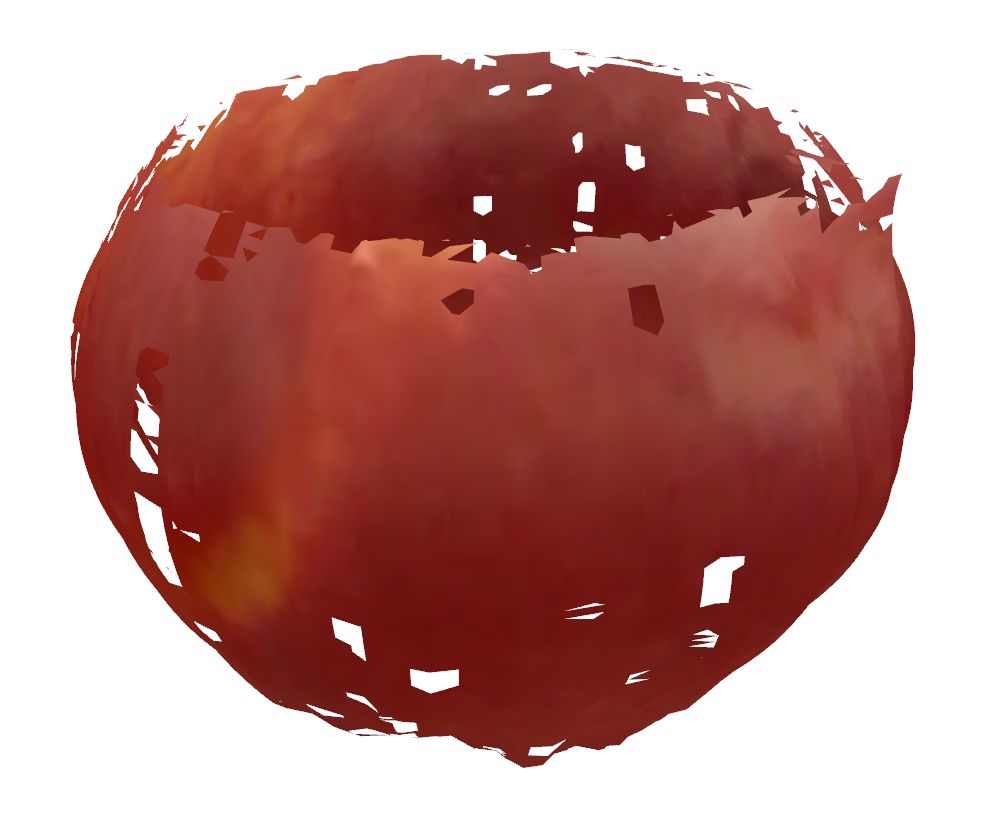
\includegraphics[scale=0.2]{bpaApple7x.PNG}
    \end{minipage}
\quad
    \begin{minipage}[b]{0.45\linewidth}
        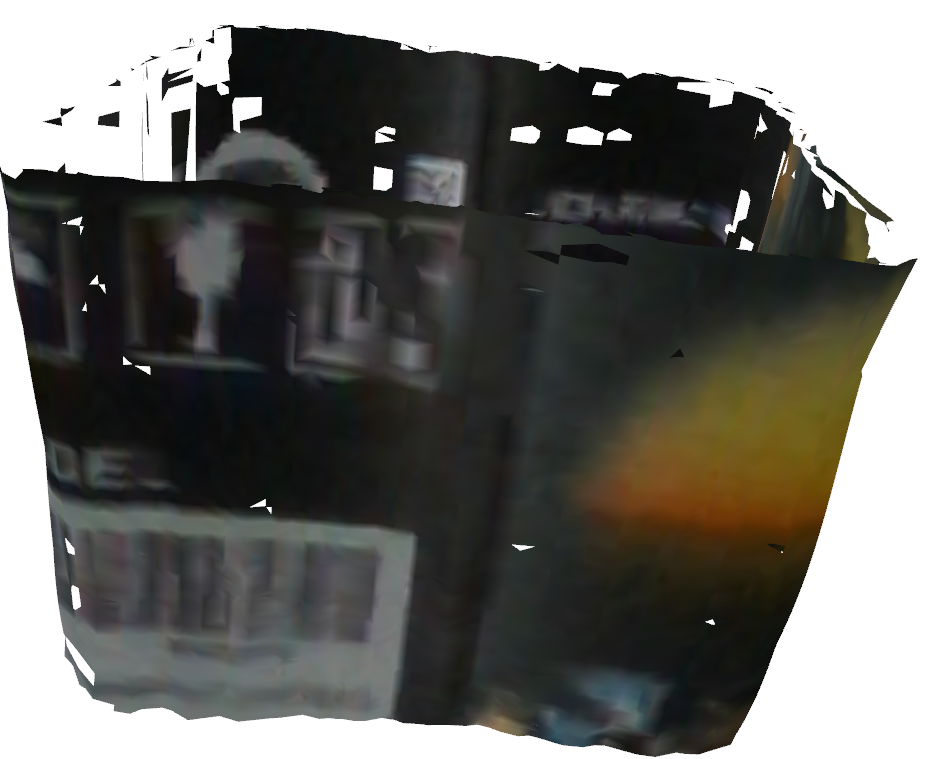
\includegraphics[scale=0.2]{bpaBox7x.PNG}
    \end{minipage}
\caption{Mesh utworzony za pomocą BPA dla jabłka oraz pudełka.}
\label{fig:appleBoxBpa}
\end{figure}

\begin{figure}[H]
  \centering
  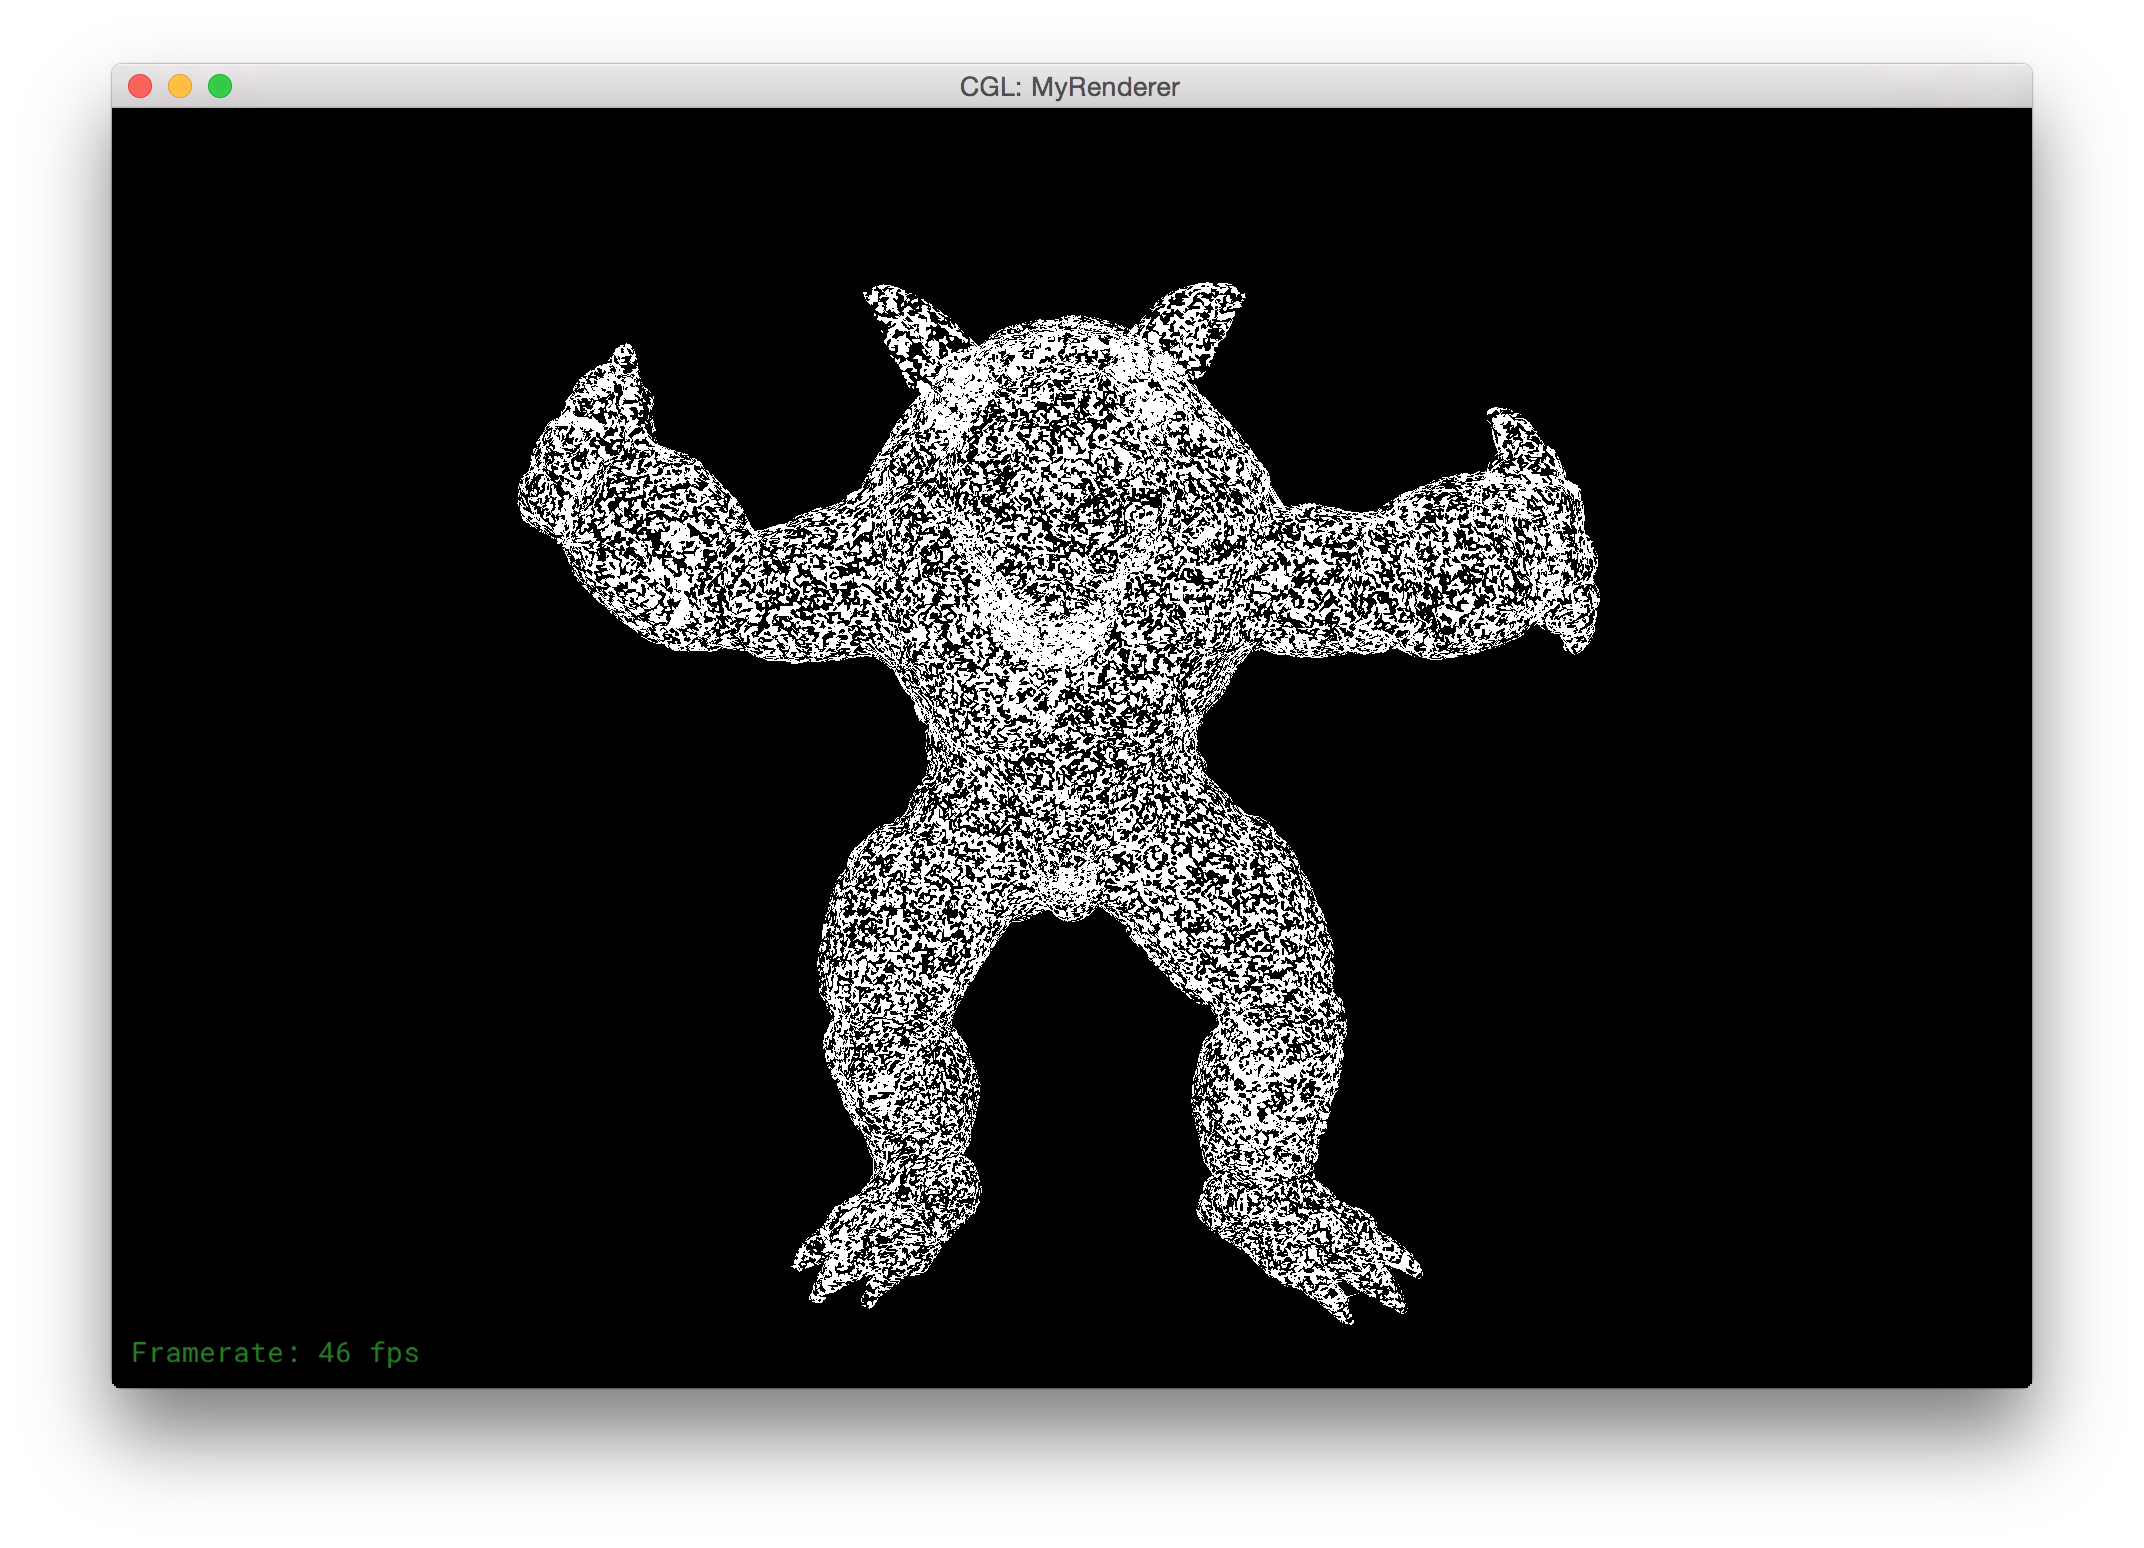
\includegraphics[scale=0.3]{armadilloBpa.png}
  \caption{Mesh człowieka armadillo wygenerowany za pomocą BPA \cite{bpaGit}.}   
  \label{fig:armadillo}
\end{figure}
W meshu człowieka Armadillo można zauważyć wiele luk. Autorzy stwierdzili, że ciężko im było dobrać odpowiedni promień kuli, dla którego powierzchnia obiektu stałaby się gładka. Na danym przykładzie widać, że algorytm BPA ma swoje wady które czasami utrudniają generację poprawnego modelu. Dla autorskich modeli również występują dziury, lecz jest ich o wiele mniej.
\newline \indent Na rysunku \ref{fig:delaAppleBoxComp} oraz \ref{fig:tetGenPicks} zestawione zostały wyniki triangulacji Delaunay'a wykonane za pomocą autorskiego programu oraz przez program TetGen firmy Wias-Berlin.

\begin{figure}[H]
\centering
    \begin{minipage}[b]{0.45\linewidth}
        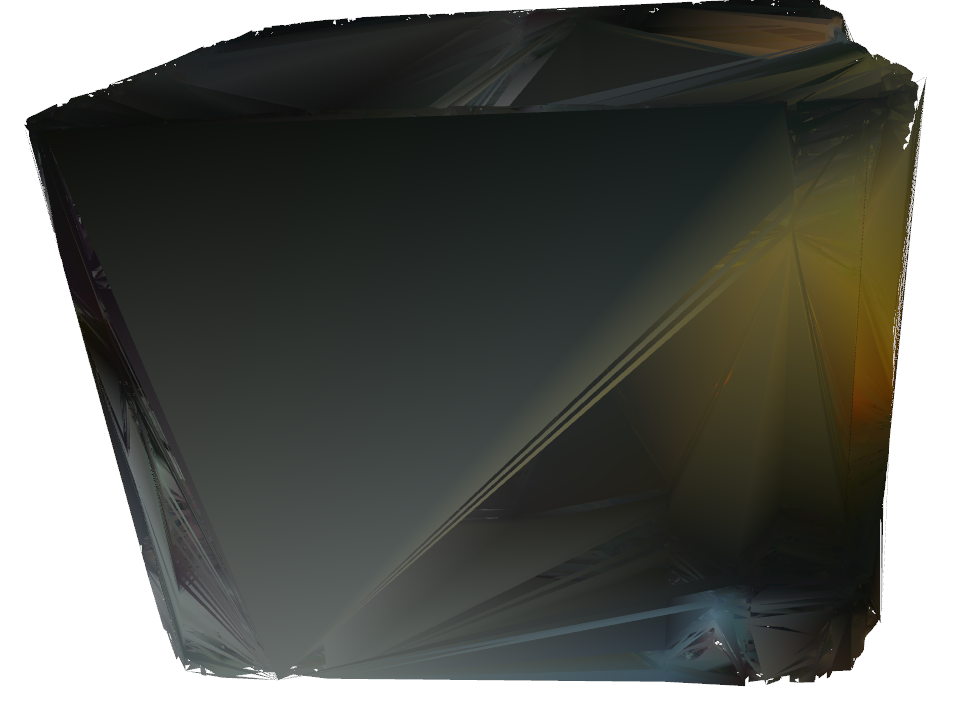
\includegraphics[scale=0.2]{delaunayBox.PNG}
    \end{minipage}
\quad
    \begin{minipage}[b]{0.45\linewidth}
        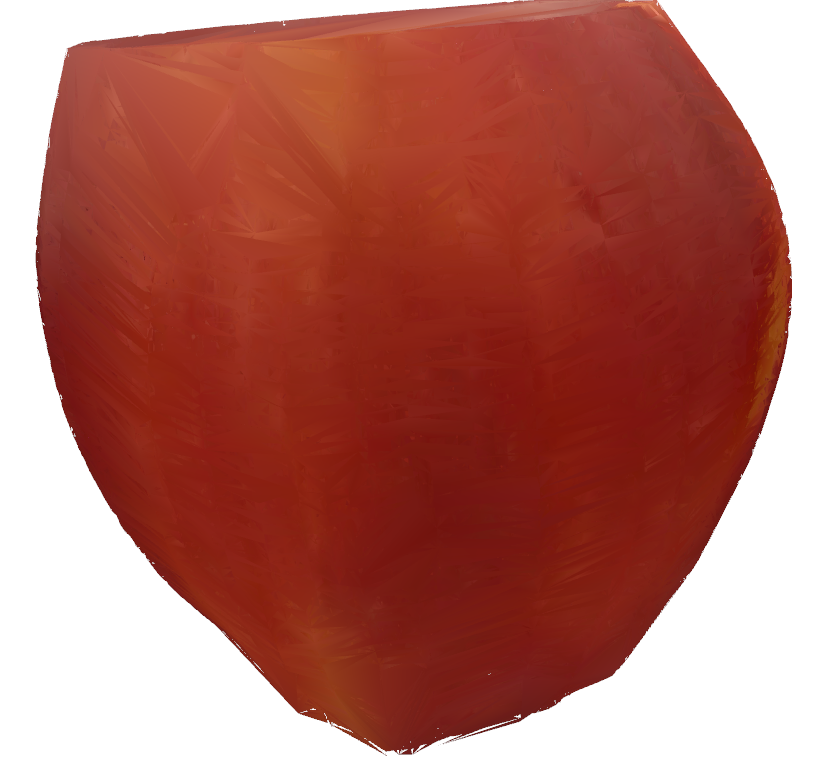
\includegraphics[scale=0.2]{jablkoDelNowe.PNG}
    \end{minipage}
\caption{Mesh utworzony za pomocą triangulacji Delaunay'a dla jabłka oraz pudełka.}
\label{fig:delaAppleBoxComp}
\end{figure}

\begin{figure}[H]
\centering
    \begin{minipage}[b]{0.45\linewidth}
        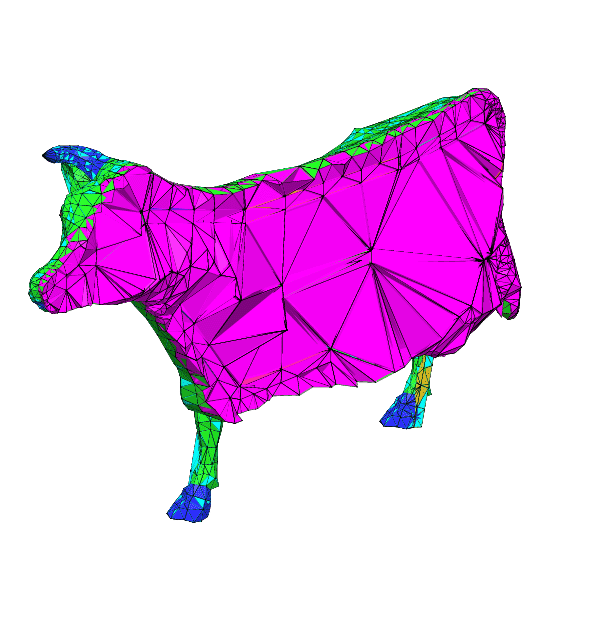
\includegraphics[scale=0.2]{cowDelIg.png}
    \end{minipage}
\quad
    \begin{minipage}[b]{0.45\linewidth}
        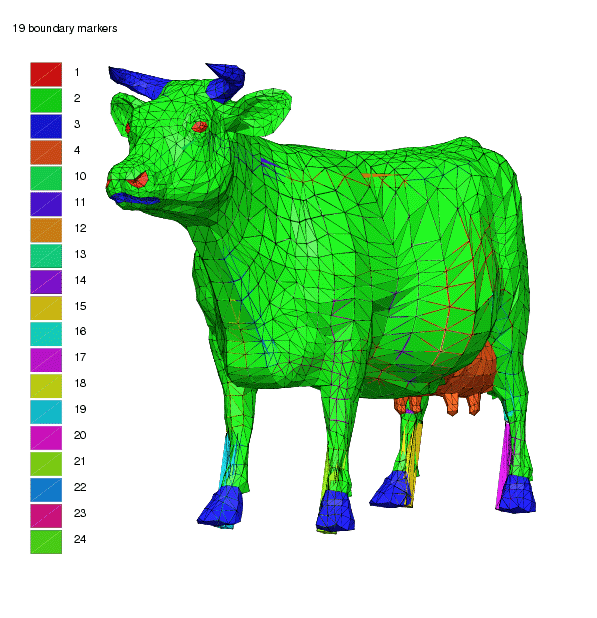
\includegraphics[scale=0.2]{cowPointsImg.png}
    \end{minipage}
\caption{Mesh triangulacji Delaunay'a oraz chmura punktów z przykładowych zdjęć programu TetGen \cite{tetGenWebsite}.}
\label{fig:tetGenPicks}
\end{figure}
Powyżej można zauważyć, że nawet obiekt wygenerowany przez profesjonalne oprogramowanie TetGen zawiera wiele niedoskonałości. Na początkowej chmurze punktów krowy, powierzchnia jest gładka. Jednak po poddaniu obróbce przez triangulację powierzchnia staje się kanciasta i zawiera wiele odstających ścian. Z kolei istotnym elementem jest brak dziur na powierzchni. Poddając modele z programu obróbce w programie Blender, można by się było pozbyć części niedoskonałości powierzchni. Porównując autorskie obiekty oraz te pochodzące z biblioteki programu firmy Wias-Berlin można dostrzec wiele podobieństw. Wynika to z użycia tego samego algorytmu, a różnice wynikają jedynie z innego podejścia do jego implementacji.


\section{Błędy oraz możliwości poprawy}
Podczas wykonywania testów zaimplementowanych metod napotkano szereg niedoskonałości. Istnieją również możliwości poprawy istniejących rozwiązań. Część z nich wynika z użytych algorytmów i metod, natomiast inne wynikają z ograniczeń sprzętowych. Poniżej przedstawione zostaną rozwiązania, których zaimplementowanie pozwoli na usprawnienie programu. Umożliwią one również zwiększenie jakości otrzymanych modeli obiektów.

Pierwszym mankamentem istniejącej metody skanowania obiektów jest brak możliwości rejestrowania przezroczystych oraz błyszczących obiektów. Wynika to z zasady działania kamery 3D. Rzutuje ona siatkę interpolacyjną na mierzony obiekt. Jednak, gdy jest on przezroczysty lub błyszczący to odbija on promień lasera. Przez dyfrakcję światła, tylko część zostaje odbita do kamery. By temu zapobiec należy użyć sprawić by obiekt odbijał mniej światła w przypadku obiektów błyszczących oraz sprawić by je odbijał w przypadku przezroczystych. By tego dokonać należy na przykład pomalować powierzchnię na matowy kolor lub przykleić taśmę. Jest to skuteczna metoda pozwalająca na akwizycję danych z tego typu obiektów. 

Kolejnym problemem który został napotkany podczas testów jest brak możliwości skanowania skomplikowanych kształtów. Jeżeli obiekt posiada wystające elementy to mogą one nie zostać zeskanowane poprawnie. W przypadku kubka, jeśli wiązka światła trafi na jego ucho, to nie zeskanuje ona tego co jest pod spodem. W efekcie na uzyskanym obiekcie będzie dostrzegalny odstający element, lecz nie to co jest pod nim. By temu zapobiec można dokonać kilku skanów, przemieszczając przy tym obiekt wzdłuż tacki. Dzięki temu jego oś obrotu zostanie przesunięta i zostanie on zeskanowany z innej strony. Dzięki temu będzie można zeskanować powierzchnię pod wystającym elementem.

Wykorzystanie metody triangulacji Delaunay'a jest bardzo kosztowne obliczeniowo. Z przeprowadzonych testów wynika, że czas trwania programu wynosi około 10 minut. Pomimo wykonania szeregu optymalizacji algorytm wciąż trwa znacznie dłużej, niż BPA dla małej długości promienia. W celu dalszej optymalizacji należy przekształcić algorytm, by wykonywał obliczenia równoległe na karcie graficznej. Kolejną możliwością jest utworzenie programu w innym języku. Utworzenie metody wykorzystującej dany algorytm w c++ pozwoli na dokonywanie szybszych obliczeń. Ten język charakteryzuje się lepszym wykorzystaniem mocy obliczeniowej procesora oraz wydajniejszym zarządzaniem pamięcią. Aktualnie język cython, pomimo tego, że jest częściowo kompilowany wciąż zawiera szereg ograniczeń wywodzących się z pythona. Poprzez zastosowanie list o nieokreślonej objętości, zarządzanie pamięcią jest mniej efektywne, a czas operacji jest dłuższy. 

Dokładność skanów jest czymś, na czym należałoby się skupić najbardziej. Istnieje wiele możliwości jej udoskonalenia. W celu zwiększenia precyzji można podnieść liczbę klatek na sekundę nagrania. Dzięki czemu zwiększone zostanie zagęszczenie punktów chmurze. Zwiększona gęstość punktów wpłynie pozytywnie na luki w algorytmie BPA. Jednocześnie przy wykorzystaniu triangulacji Delauny'a gęstsze rozmieszczenie punktów w chmurze wpływa na zmniejszenie wielkości ścian generowanych trójkątów. Gdy pola trójkątów interpolacyjnych będą mniejsze, to będą one siebie nawzajem mniej zakrywać. Poprzez taki zabieg, tekstura obiektu zostanie wierniej oddana. Zmniejszając prędkość obrotową tacki można uzyskać ten sam rezultat, co w przypadku zwiększania liczby klatek. Przy wolniejszym ruchu tacki, wykonane zostanie więcej zdjęć. Wydaje się to być lepszym rozwiązaniem, ponieważ prędkość transmisji danych przez protokół USB nie będzie już ograniczeniem, wzrośnie jedynie czas pomiaru. Znaczną poprawę może również wnieść zmiana sposobu akwizycji danych o głębi. Z przeprowadzonych analiz wynika, że skaner liniowy lepiej oddaje powierzchnię modelu niż metoda światła strukturalnego. Jednakże wprowadzenie dodatkowych przekształceń do tej metody, mogłoby skutkować zwiększeniem jakości generowanych chmur punktów. Kolejnym sposobem na zwiększenie dokładności modeli jest ekstrapolacja kolumn. W tym celu należy w puste przestrzenie pomiędzy kolejnymi kolumnami dodać nowe. Dokonanie tego będzie możliwe dzięki wykorzystaniu pozycji wcześniejszych punktów. Uśrednione pozycje dwóch sąsiednich punktów będą stanowić pozycję środkowego. Dana operacja może zostać wykonana wielokrotnie. Zwiększy to zagęszczenie punktów, jednak mogą zaistnieć przekłamania. Pomiędzy kolumnami występują efekty nieuchwytne, które są niemożliwe do wyznaczenia. W miejscu gdzie nie znajduje się żaden punkt mogło na przykład być wgłębienie. Przy ekstrapolacji zostanie ono jednak zastąpione uśrednioną wartością z okolicznych punktów. Najlepszym rozwiązaniem wydaje się być wykonanie dodatkowych skanów. Należy zarejestrować w jakich miejscach nastąpiły przekłamania punktów, a następnie uruchomić ponownie skan. Można również zarejestrować kilka pełnych obrotów tacki. Posiadając kilka ujęć tego samego kąta obrotu, będzie można wybrać tę wartość która nie jest przekłamana. Poprzez taki zabieg będzie można uniknąć aktualnie dokonywanej interpolacji punktów. Znane wówczas będą rzeczywiste pozycje punktów, a modele w ten sposób wygenerowane będą wierniej odwzorowywały rzeczywistość. 
 
Ostatnim widocznym w testach ograniczeniem aktualnie wykorzystywanej metody skanowania trójwymiarowego jest brak górnej oraz dolnej ściany. Wykonując skan od boku, nie ma możliwości wyznaczenia kształtu górnej oraz dolnej ściany. Pierwszym sposobem uniknięcia tego jest wykonanie skanu z różnych perspektyw, a następnie nałożenie różnych części modelu na siebie w programie Blender. Będzie to jednak bardzo skomplikowane, ponieważ należy dokonać ekstrakcji jedynie potrzebnych płaszczyzn. Innym sposobem jest wykonanie skanu pod kątem. Dzięki takiemu zabiegowi, oprócz ścian bocznych zarejestrowana zostanie też ściana górna. Jednakże  taki zabieg znacząco utrudnia przekształcenia geometryczne. Oprócz już istniejących będzie należało dodać dodatkowe, uwzględniające przesunięcie kamery oraz jej kąt względem obiektu.
\newpage






\renewcommand{\listtablename}{Spis tabel}
\renewcommand{\listfigurename}{Spis rysunków}
\addcontentsline{toc}{chapter}{Spis tabel}
\addcontentsline{toc}{chapter}{Spis rysunków}
\listoffigures
\listoftables


\addcontentsline{toc}{chapter}{Bibliografia}
\bibliography{references}
\bibliographystyle{ieeetr}
\end{document}
